\documentclass{article}
\usepackage[utf8]{inputenc}

\title{Elliptic Curves, Complex Tori, Modular Forms, and $\ell$-adic Galois Representations}
\author{Benjamin Church}

\usepackage[english]{babel}
\usepackage[a4paper, total={6in, 9in}]{geometry}
\usepackage{tikz-cd}
\usepackage{graphicx}
\usepackage{float}
 
\usepackage{amsthm, amssymb, amsmath, centernot}

\newcommand{\into}{\hookrightarrow}
\newcommand{\Gal}[1]{\mathrm{Gal}\left( #1 \right)}
\newcommand{\Aut}[1]{\mathrm{Aut} \small(#1 \small)}
\newcommand{\SL}[0]{\mathrm{SL}}
\newcommand{\End}[0]{\mathrm{End}}
\newcommand{\GL}[2]{\mathrm{GL}_{#1}\left(#2\right)}
\newcommand{\SO}[0]{\mathrm{SO}}
\newcommand{\Rept}[0]{\mathrm{Re}}
\newcommand{\Impt}[0]{\mathrm{Im}}
\newcommand{\dv}[0]{\mathrm{div}}
\newcommand{\Dv}[0]{\mathrm{Div}}
\newcommand{\Og}[0]{\mathit{\Omega}}
\newcommand{\og}[0]{\mathit{\omega}}

\newcommand{\notimplies}{%
  \mathrel{{\ooalign{\hidewidth$\not\phantom{=}$\hidewidth\cr$\implies$}}}}
 
\renewcommand\qedsymbol{$\square$}
\newcommand{\cont}{$\boxtimes$}
\newcommand{\divides}{\mid}
\newcommand{\ndivides}{\centernot \mid}
\newcommand{\Z}{\mathbb{Z}}
\newcommand{\R}{\mathbb{R}}
\newcommand{\Q}{\mathbb{Q}}
\newcommand{\N}{\mathbb{N}}
\newcommand{\C}{\mathbb{C}}
\newcommand{\Zplus}{\mathbb{Z}^{+}}
\newcommand{\Primes}{\mathbb{P}}
\newcommand{\colim}[1]{\mathrm{colim}(#1)}
\newcommand{\Ob}[1]{\mathrm{Ob}(#1)}
\newcommand{\cat}[1]{\mathcal{#1}}
\newcommand{\id}{\mathrm{id}}
\newcommand{\Hom}[2]{\mathrm{Hom}\left( #1, #2 \right)}
\newcommand{\catHom}[3]{\mathrm{Hom}_{#1}\left( #2, #3 \right)}
\newcommand{\Top}{\mathbf{Top}}
\newcommand{\pTop}{\mathbf{Top}_{\bullet}}
\newcommand{\Set}{\mathbf{Set}}
\newcommand{\pSet}{\mathbf{Set}_\bullet}
\newcommand{\hTop}{\mathbf{hTop}}
\newcommand{\phTop}{\mathbf{hTop}_{\bullet}}
\renewcommand{\Im}[1]{\mathrm{Im}(#1)}
\newcommand{\homspace}[2]{\left< #1, #2 \right>}
\newcommand{\rp}{\mathbb{RP}}
\newcommand{\coker}[1]{\mathrm{coker}\: #1}

\renewcommand{\d}[1]{\: \mathrm{d}#1 \:}
\newcommand{\dn}[2]{\: \mathrm{d}^{#1} #2 \:}
\newcommand{\deriv}[2]{\frac{\d{#1}}{\d{#2}}}
\newcommand{\nderiv}[3]{\frac{\dn{#1}{#2}}{\d{#3^2}}}
\newcommand{\pderiv}[2]{\frac{\partial{#1}}{\partial{#2}}}
\newcommand{\parsq}[2]{\frac{\partial^2{#1}}{\partial{#2}^2}}
\newcommand{\Imt}[0]{\mathrm{Im}}

\theoremstyle{definition}
\newtheorem{theorem}{Theorem}[section]
\newtheorem{lemma}[theorem]{Lemma}
\newtheorem{proposition}[theorem]{Proposition}
\newtheorem{example}[theorem]{Example}
\newtheorem{corollary}[theorem]{Corollary}
\newtheorem{remark}{Remark}[section]
\newtheorem{problem}{Problem}

\newenvironment{definition}[1][Definition:]{\begin{trivlist}
\item[\hskip \labelsep {\bfseries #1}]}{\end{trivlist}}


\newenvironment{lproof}{\begin{proof} \renewcommand{\qedsymbol}{}}{\end{proof}}
\renewcommand{\mod}[3]{\: #1 \equiv #2 \: (\text{mod} \: #3)}
\newcommand{\nmod}[3]{\: #1 \centernot \equiv #2 \: mod \: #3 \:}
\newcommand{\ndiv}{\hspace{-4pt}\not \divides \hspace{2pt}}
\newcommand{\gen}[1]{\langle #1 \rangle}
\newcommand{\hook}{\hookrightarrow}
\newcommand{\Tor}[4]{\mathrm{Tor}^{#1}_{#2} \left( #3, #4 \right)}
\newcommand{\Ext}[4]{\mathrm{Ext}^{#1}_{#2} \left( #3, #4 \right)}

\tikzset{
    labl/.style={anchor=south, rotate=90, inner sep=.5mm}
}

\renewcommand{\bf}[1]{\mathbf{#1}}
\newcommand{\Class}[2]{\mathcal{C}^{#1} \left( #2 \right)}
\newcommand{\Res}[2]{\mathrm{Res}_{#1} \: #2}
\newcommand{\F}{\mathcal{F}}
\newcommand{\G}{\mathcal{G}}
\renewcommand{\O}{\mathcal{O}}
\newcommand{\iO}{\mathcal{O}}
\newcommand{\finfield}[1]{\mathbb{F}_{#1}}

\renewcommand{\S}[1]{\mathcal{S}_{#1}}
\newcommand{\M}[1]{\mathcal{M}_{#1}}
\newcommand{\E}[1]{\mathcal{E}_{#1}}

\newcommand{\h}{\mathfrak{h}}
\newcommand{\MG}{\SL_2(\Z)}

\renewcommand{\P}[2]{\mathbb{P}^{#1} \left( #2 \right)}

\begin{document}

\maketitle

\tableofcontents

\newpage

\section{Introduction}

Elliptic curves are one of the most important objects in modern mathematics. They provide a clear link between geometry, number theory, and algebra. Such objects appear naturally in the study of Diophantine equations and of complex analysis and are vital to the proofs of many famous theorems in number theory such as Fermat's Last theorem. Elliptic curves are so-called one-dimensional projective varieties of genus one meaning they are curves living in projective space defined by a cubic equation.

\begin{definition}
Let $K$ be a field then $n$-dimensional projective space over $K$ is defined by,
\[ \P{n}{K} = (K^{n+1} \setminus \{ 0 \}) / K^{\times} \]
We write the coordinates as,
\[ [X_0 : \cdots : X_n] = [\lambda X_0 : \cdots : \lambda X_n] \]
where $\lambda \in K^\times$.
\end{definition}

\begin{definition}
An \textit{elliptic curve} $E$ defined over a field $K$ is a smooth projective curve defined by the inhomogeneous equation,
\[ y^2 = x^3 + a x + b \]
for $a,b \in K$, that is, for any field $L / K$, we define,
\[ E(L) = \left\{ (x,y) \in L^2 \mid y^2 = x^3 + ax + b \right\} \cup \left\{ O \right\} \subset L^2 \]
The distinguished point $O$ is viewed as the ``point at infinity.'' We can express $E$ as a projective curve in $\P{3}{L}$ by the homoegenized equation,
\[ ZY^2 - X^3 - a Z^2 Y - b Z^3 = 0 \]
where we identify the points with $Z \neq 0$ such that,
\[ [X : Y : Z] = [ X/Z : Y/ Z : 1]  \]
with $(x, y)$ for $x = X/Z$ and $y = Y/Z$. Furthermore we identify the unique point $[X : Y : 0]$ on $E$ with $O$. 
Usually, we will either take $K$ to be algebraically closed or define the points $E$ to be $E(\bar{K})$ where $\bar{K}$ denotes the algebraic closure, then $E(L) = E \cap L$ which is exactly the set of fixed points of $E$ under the action of $\Gal{\bar{K}/L}$. 
\end{definition}
We will return to the geometric development of elliptic curves. However, we will begin with the complex analyic picture in which an elliptic curve will, somewhat suprisingly, naturally arise. 

\section{Elliptic Functions}

On the real line, analytic periodic functions like sinusoids have wonderful properties are are intimately related to the points quadratic curves i.e. circles. We might naturally ask: ``what is the analogue of a periodic function on the complex plane?'' The following is one such notion.

\begin{definition}
A function $f : \C \to \C$ is \textit{doubly periodic} or \textit{elliptic} if there exits two independent (not real multiples of each other) complex numbers $\omega_1$ and $\omega_2$ such that,
\[ f(z + \omega_1) = f(z) \quad \text{and} \quad f(z + \omega_2) = f(z) \]
We define the lattice of periods,
\[ \Lambda = \{ n \omega_1 + m \omega_2 \mid n,m \in \Z \} \]
so that $f(z + \omega) = f(z)$ for all $\omega \in \Lambda$ so $f$ factors as a function on the quotient $f : \C / \Lambda \to \C$. 
\end{definition}

\begin{remark}
The space $\C / \Lambda$ is topologically a torus. It is equivalent to the ``fundamental parallelogram''
\[ \{ \alpha \omega_1 + \beta \omega_2 \mid \alpha, \beta \in [0, 1] \} \]
with opposite edges identified. This is the standard construction of a torus. However, different lattices $\Lambda$ will put a different complex structure on $\C / \Lambda$ which we therefore call a complex torus. 
\end{remark}
\noindent
We would want to consider elliptic homomorphic functions. However, a classical theorem in complex analysis poses a difficulty.

\begin{theorem}[Liouville]
Every bounded entire\footnote{holomorphic on the entire complex plane} function is constant.
\end{theorem}

\begin{proof}
Let $f : \C \to \C$ be entire and bounded everywhere by $M$. Take $w \in \C$ and let $C$ be a circle arround $z$ with radius $R$. Then applying the Cauchy integral formula,
\[ f'(w) = \frac{1}{2 \pi i} \oint_C \frac{f(z)}{(z - w)^2} \d{z} = \frac{1}{2 \pi} \int_0^{2 \pi} \frac{f(w + R e^{i \theta})}{R^2 e^{2 i \theta}} R \d{\theta} \]
Therefore,
\[ |f'(w)| = \frac{1}{2 \pi} \left| \oint_C \frac{f(z)}{(z - w)^2} \d{z} \right| \le \frac{1}{2 \pi} \int_0^{2 \pi} \frac{|f(w + R e^{i \theta})|}{R^2} R \d{\theta} \le \frac{1}{2 \pi} \int_0^{2 \pi} \frac{M}{R} \d{\theta} = \frac{M}{R} \]
which goes to zero in the limit $R \to \infty$. Since $R$ is arbitrarily large, $f'(w) = 0$ so $f$ is constant since it has zero derivative everywhere. 
\end{proof}

\begin{corollary}
There do not exist nonconstant doubly periodic holomorphic functions.
\end{corollary}

\begin{proof}
Suppose that $f : \C \to \C$ is holomorphic and doubly periodic with periods $\omega_1$ and $\omega_2$. Consider $f$ restricted to the so-called ``fundamental domain''
\[ D = \{ \alpha \omega_1 + \beta \omega_2 \mid \alpha, \beta \in [0, 1] \} \]
By using the periodicity, the behavior of $f$ everywhere is determined by its values on $D$. 
Since $D$ is compact\footnote{closed and bounded for subsets of Euclidean space} and $f$ is continuous (since it is holomorphic) it must be bounded\footnote{A continuous function on a compact set cannot diverge approaching a point because the set is closed nor diverge off to infinity because the set is bounded.} on $D$. Therefore, $f$ is entire and bounded and thus, by Liouville's theorem, constant. 
\end{proof}
Our plan has been thwarted as soon as it was devised. Since we cannot find interesting holomorphic examples of elliptic functions we now ask for the next best thing.
We want to consider elliptic meromorphic functions. That is, meromorphic functions $f : \C / \Lambda \to \C$. It turns out that now were are in luck. A canonical example of a meromorphic function is $z^{-2}$. We will try to make such a function periodic. A standard trick is to sum over the entire lattice such that shifts by lattice elements do not effect the sum. We might try,
\[ f(z) = \sum_{\omega \in \Lambda} \frac{1}{(z + \omega)^2} \] 
which is doubly periodic because if $\omega \in \Lambda$ then,
\[ f(z + \omega) = \sum_{\omega' \in \Lambda} \frac{1}{(z + \omega + \omega')^2} = \sum_{\omega'' \in \Lambda} \frac{1}{(z + \omega'')^2} = f(z) \]
However, this definition has one major flaw. That sum does not converge! To fix this, we use a clever subtraction to remove the divergent part of the sum and arrive at the following definition by Weierstrass. 
\begin{theorem}
Let $\Lambda \subset \C$ be a Lattice. The Weierstrass $\wp$-function, defined as,
\[ \wp(z) = \frac{1}{z^2} + \sum_{\omega \in \Lambda^\times } \left[ \frac{1}{(z + \omega)^2} - \frac{1}{\omega^2} \right] \]
is a well-defined meromorphic function $\wp : \C / \Lambda \to \C$ with double poles on $\Lambda$. 
\end{theorem}

\begin{proof}
We can write,
\begin{align*} 
\frac{1}{(z + \omega)^2} & = - \deriv{}{z} \left( \frac{1}{z + \omega} \right) = - \frac{1}{\omega} \deriv{}{z} \left[ \sum_{n = 0}^\infty \left( - \frac{z}{\omega} \right)^n \right] = - \frac{1}{\omega} \sum_{n = 0}^\infty \left[ \frac{ (-1)^n n z^{n-1}}{\omega^{n}} \right] 
\\
& = \frac{1}{\omega^2} \left[ \sum_{n = 0}^\infty (-1)^n (n + 1) \frac{z^n}{\omega^n} \right]  
\end{align*}
and this series is uniformly convergent for $|z| < |\omega|$. Thus,
\[ \frac{1}{(z + \omega)^2} - \frac{1}{\omega^2} = \frac{1}{\omega^2} \sum_{n=1}^\infty (-1)^n (n+1) \frac{z^n}{\omega^n} \]
and therefore, 
\[ \wp(z) = \frac{1}{z^2} + \sum_{\omega \in \Lambda^\times} \left[ \frac{1}{(z + \omega)^2} - \frac{1}{\omega^2} \right] \]
converges uniformly. Furthermore, 
\[ \wp'(z) = - \frac{2}{z^3} + \sum_{\omega \in \Lambda^\times} \left( - \frac{2}{(z + \omega)^3} \right) = - 2 \sum_{\omega \in \Lambda} \frac{1}{(z + \omega)^3} \]
Thus, $\wp'(z)$ is doubly periodic with periods $\omega_1$ and $\omega_2$. Thus, $\wp(z + \omega_1) = \wp(z) + c_1$ so $\wp(-\tfrac{1}{2} z_1) = \wp(\tfrac{1}{2} z) + c_1$ but $\wp$ is even so $c_1 = 0$. The same for $\omega_2$. Thus, $\wp(z + \omega_1) = \wp(z)$ and $\wp(z + \omega_2) = \wp(z)$. 
\end{proof}


\subsection{The Defining Differential Equation for $\wp$}

We need to work out he expansion for $\wp(z)$ near $0$. We have,
\[ \frac{1}{(z - \omega)^2} = \frac{1}{\omega^2} \cdot \frac{1}{(1 - \frac{z}{\omega})^2} = \frac{1}{\omega^2} \sum_{n = 0}^\infty (m + 1) \left( \frac{z}{\omega} \right)^m \]
Therefore,
\begin{align*}
\wp(z) &= \frac{1}{z^2} + \sum_{\omega \in \Lambda^\times} \sum_{m = 1}^\infty (m + 1) \frac{z^{m}}{\omega^{m + 2}} 
\\
& = \frac{1}{z^2} + \sum_{m = 1}^\infty (m + 1) z^m \left( \sum_{\omega \in \Lambda^\times} \frac{1}{\omega^{m+2}} \right) 
\\
& = \frac{1}{z^2} + \sum_{k = 1}^\infty (2 k + 1) z^{2k} G_{k+1}(\Lambda) 
\end{align*}
where we have defined,
\[ G_{k}(\Lambda) = \sum_{\omega \in \Lambda^\times} \frac{1}{\omega^{2k}} \] 
The odd terms vanish because if we sum an odd function over the lattice then we get zero. 
Explicitly,
\begin{align*}
\wp(z) = \frac{1}{z^2} + 3 G_2(\Lambda) z^2 + 5 G_3(\Lambda) z^4 + O(z^6) 
\end{align*}
Next,
\[ \wp'(z) = - \frac{2}{z^3} + \sum_{k = 1}^\infty (2 k + 1) (2k) G_{k+1}(\Lambda) z^{2k - 1} \]
which we sum as,
\[ \wp'(z) = - \frac{2}{z^3} + 6 G_2(\Lambda) z + 20 G_3(\Lambda) z^3 + O(z^5) \]
Thus, compute,
\begin{align*}
\wp'(z)^2 & = \left(  - \frac{2}{z^3} + 6 G_2(\Lambda) z + 20 G_3(\Lambda) z^3 + O(z^5) \right)^2 
\\
& = \frac{4}{z^6} - 24 G_2(\Lambda) \frac{1}{z^2} - 80 G_3(\Lambda) + O(z^2) 
\end{align*}
Similarly, compute,
\begin{align*}
\wp(z)^3 & = \left( \frac{1}{z^2} + 3 G_2(\Lambda) z^2 + 5 G_3(\Lambda) z^4 + O(z^6) \right)^3
\\
& = \frac{1}{z^6} + 9 G_2(\Lambda) \frac{1}{z^2} + 15 G_3(\Lambda) + O(z^2) 
\end{align*}
Therefore,
\begin{align*}
\wp'(z)^2 - 4 \wp(z)^3 & = - 24 G_2(\Lambda) \frac{1}{z^2} - 36 G_2(\Lambda) \frac{1}{z^2} - 80 G_3(\Lambda) - 60 G_3(\Lambda) + O(z^2) 
\\
& = - 60 G_2(\Lambda) \frac{1}{z^2} - 140 G_3(\Lambda) + O(z^2)
\end{align*}
Which implies that,
\begin{align*}
\wp'(z)^2 - 4 \wp(z)^3 + 60 G_2(\Lambda) \wp(z) + 140 G_3(\Lambda) = O(z^2)
\end{align*}
Therefore the function,
\[ \wp'(z)^2 - 4 \wp(z)^3 + 60 G_2(\Lambda) \wp(z) + 140 G_3(\Lambda) \]
is holomorphic on $\C$ and is doubly periodic and thus constant. However, it vanishes at $z = 0$ and thus must be the zero function. Therefore, we have the differential equation,
\[ \wp'(z)^2 - 4 \wp(z)^3 + 60 G_2(\Lambda) \wp(z) + 140 G_3(\Lambda)  = 0 \]
We can interpret this differential equation as telling us that the image of the elliptic Weierstrass $\wp$-function lies on a special type of object called an elliptic curve.  

\begin{definition}
An \textit{elliptic curve} $E$ defined over a field $K$ is a smooth projective curve defined by the inhomogeneous equation,
\[ y^2 = x^3 + a x + b \]
for $a,b \in K$, that is, for any field $L / K$, we define,
\[ E(L) = \left\{ (x,y) \in L^2 \mid y^2 = x^3 + ax + b \right\} \cup \left\{ O \right\} \subset L^2 \]
The distinguished point $O$ is viewed as the ``point at infinity.'' We can express $E$ as a projective curve in $\P{3}{L}$ by the homoegenized equation,
\[ ZY^2 - X^3 - a Z^2 Y - b Z^3 = 0 \]
where we identify the points with $Z \neq 0$ such that,
\[ [X : Y : Z] = [ X/Z : Y/ Z : 1]  \]
with $(x, y)$ for $x = X/Z$ and $y = Y/Z$. Furthermore we identify the unique point $[X : Y : 0]$ on $E$ with $O$. 
Usually, we will either take $K$ to be algebraically closed or define the points $E$ to be $E(\bar{K})$ where $\bar{K}$ denotes the algebraic closure, then $E(L) = E \cap L$ which is exactly the set of fixed points of $E$ under the action of $\Gal{\bar{K}/L}$. 
\end{definition}
Define $g_2 = 60 G_2(\Lambda)$ and $g_3 = 140 G_3(\Lambda)$. Then we have the fundamental differential equation,
\[ \wp'(z)^2 = 4 \wp(z)^3 - g_2 \wp(z) - g_3 \] 
Let $E$ be the Elliptic curve over $\C$ defined by the equation,
\[ y^2 = x^3 - (g_2/4) x - (g_3/4) \]
then, we see that the Weierstrass $\wp$-function gives a map to this elliptic curve $\Phi_{\wp} : \C / \Lambda \to E$ given by,
\[ z \mapsto [\wp(z), \wp'(z)/2, 1] \]
unless $\wp(z)$ has a pole at $z$ i.e. $z \in \Lambda$ in which case we send $z$ to the ``point at infinity'' via $z \to [0 : 1 : 0]$.

\subsection{Inverse to the Abel Map} 

The defining differential equation implies that,
\begin{align*}
\int_{0}^{z} \frac{\wp'(z) \d{z}}{\sqrt{4 \wp(z)^3 - g_2 \wp(z) - g_3}} = z 
\end{align*}
Let $u = \wp(z)$ then we have,
\[ \int_{\infty}^{\wp(z)} \frac{\d{u}}{\sqrt{4 u^3 - g_2 u - g_3}} = z\]
Thus if we introduce the elliptic integral,
\[ E(v) = \int_{\infty}^v \frac{\d{u}}{\sqrt{4 u^3 - g_2 u - g_3}} \]
then we have,
\[ E(\wp(z)) = z \]
This elliptic function is known as the Abel map on the elliptic curve. I claim that the Wierstass $\wp$-function gives a bijection between the complex points of $E$ and the torus $\C / \Lambda$ because the elliptic integral provides an inverse.

\section{The Group Law}

The truly remarkable thing about the identification via the Weierstrass $\wp$-function of the complex torus $\C / \Lambda$ with the complex points of an elliptic curve is that the complex torus $\C / \Lambda$ naturally has an abelian group structure under the usual addition of complex numbers modulo $\Lambda$. This allows us to define an abelian group structure on $E$ as follows. For points $P, Q \in E$, define the analytic group law via,
\[ P + Q = \Phi_{\wp}(\Phi^{-1}_{\wp}(P) + \Phi^{-1}_{\wp}(Q)) \]
where ``+'' on the right denotes the usual addition of complex numbers in $\C / \Lambda$. This abelian group law turns $E$ into a very special type of algebraic geometric object called an \textit{abelian variety}. 
\bigskip\\
Now we should investigate the possible geometric interpretations of such a group operation on $E$.

\begin{lemma}
A line intersects a planar cubic curve at exactly three points (counting multiplicity). 
\end{lemma}

\begin{proof}
The linear equation alows us to write $y$ in terms of $x$. Then the defining equation of the cubic curve reduces to a cubic in $x$ which has exactly three solutions. 
\end{proof}

\begin{remark} 
We define the points of the curve $E$ always over $\bar{K}$, the algebraic closure, to ensure that there are always enough solutions.
\end{remark}

\begin{definition}
Let $E$ be an elliptic curve. The \textit{geometric group law} on $E$ with a distinguished point $O$ is defined as follows. For $P,Q \in E$, take the third intersection point $P * Q$, join
it to $O$ by a line, and then take the third intersection point to
be $P + Q$. In other words, set $P + Q = O * (P * Q)$. In the case that $P = Q$ we define $P * P$ by taking the tangent line at $P$ and the thrid point where it intersects $E$. The necessity that each point have a well-defined tangent line is one reason we restrict elliptic curves to \textit{nonsingular} cubic curves. 
\begin{figure}[H]
\begin{center}
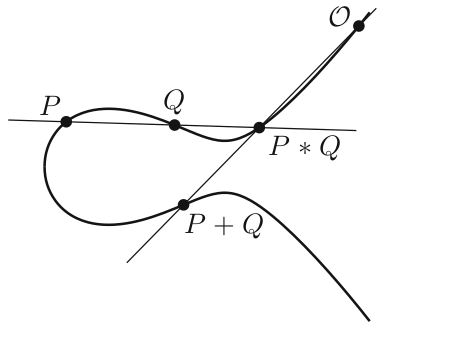
\includegraphics[scale=0.5]{EC1}
\caption{The illustration of addition of \textit{real} points on an elliptic curve.}
\end{center}
\end{figure}
\end{definition}

\begin{lemma}
We have $P * Q = Q * P$ and $P * (P * Q) = Q$.
\end{lemma}

\begin{proof}
Clearly the lines $PQ$ and $QP$ are the same and thus intersect $E$ at the same additional point.
Let $S = P * Q$ then $P$, $Q$, and $S$ are all three points that the line $PQ = QS = SP$ intersect $E$ at. Thus, $P * S = Q$ since it is the third intersection point.
\end{proof}

\begin{proposition}
The geometric group law on $E$ with respect to $O$ has identity $O$, is commutative, and admits an inverse, denoted $-P$ for each point $P$.
\end{proposition}

\begin{proof}
We have $P + O = O * (P * O) = P$. Futhermore, $P * Q = Q * P$ which implies that $P + Q = Q + P$.
\begin{figure}[H]
\begin{center}
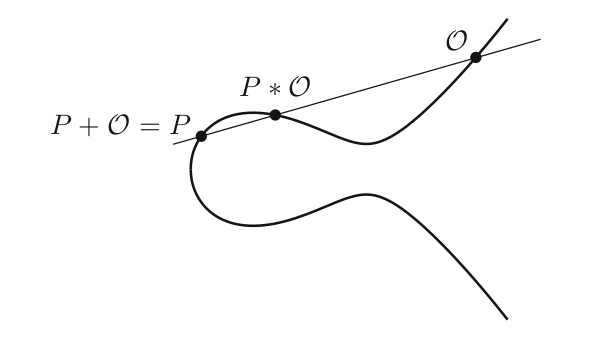
\includegraphics[scale=0.5]{EC2}
\caption{The illustration of the identity on the \text{real} points on an elliptic curve.}
\end{center}
\end{figure}
Next, let $S = O * O$ then define $-P = P * S$. We have, $P + (-P) = O * (P * (P * S))$. However, $P * (P * S) = S$ so $P + (-P) = O * S = O * (O * O) = O$. 
\begin{figure}[H]
\begin{center}
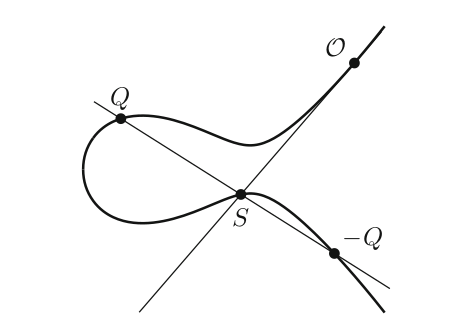
\includegraphics[scale=0.5]{EC3}
\caption{The illustration of inversion of a \text{real} point on an elliptic curve.}
\end{center}
\end{figure}
\end{proof}

\begin{lemma}
Let $C_1$ and $C_2$ be two cubic curves which intersect generically at 9 points. Suppose a cubic curve $C$ intersects $C_1$ and $C_2$ at eight of the points then $C$ intersects $C_1$ and $C_2$ at all 9 points. 
\end{lemma}

\begin{proof}
A generic cubic curve is defined by nine coefficients. The requirement that $C$ intersect $C_1$ and $C_2$ at eight points gives eight constraint equations which limit the space of possible curves to a one-dimensional family. Let $F_1(x, y) = 0$ and $F_2(x, y) = 0$ be cubic equations defining $C_1$ and $C_2$ then $\lambda_1 F_1(x,y) + \lambda_2 F_2(x,y) = 0$ for arbitrarly $\lambda_1$ and $\lambda_2$ is at least a one-dimensional family of curves which all pass through the eight defining points. Thus every curve $C$ must be one of these. However, since $C_1$ and $C_2$ both pass throught the nineth point $F_1$ and $F_2$ vanish there and thus so does $\lambda_1 F_1(x,y) \lambda_2 F_2(x,y)$ which implies that $C$ also passes through the last intersection point. 
\end{proof}

\begin{proposition}
The geometric group law is associative. Therefore, $(E, O, +)$ is an abelian group. 
\end{proposition}

\begin{proof}
Let $P,Q,R \in E$ be three points on the elliptic curve. Then consider the eight points, 
\[ O, \: P, \: Q, \: R, P * Q, \: P + Q, \: Q * R, \: Q + R\]
which lie on $E$ and a nineth point $N$ which is the intersection of the lines $(P + Q) R$ and $P(Q + R)$. We want to show that this last point lies on $E$ such that $(P + Q) * R = P * (Q + R)$ which implies that $(P + Q) + R = P + (Q + R)$.
\begin{figure}[H]
\begin{center}
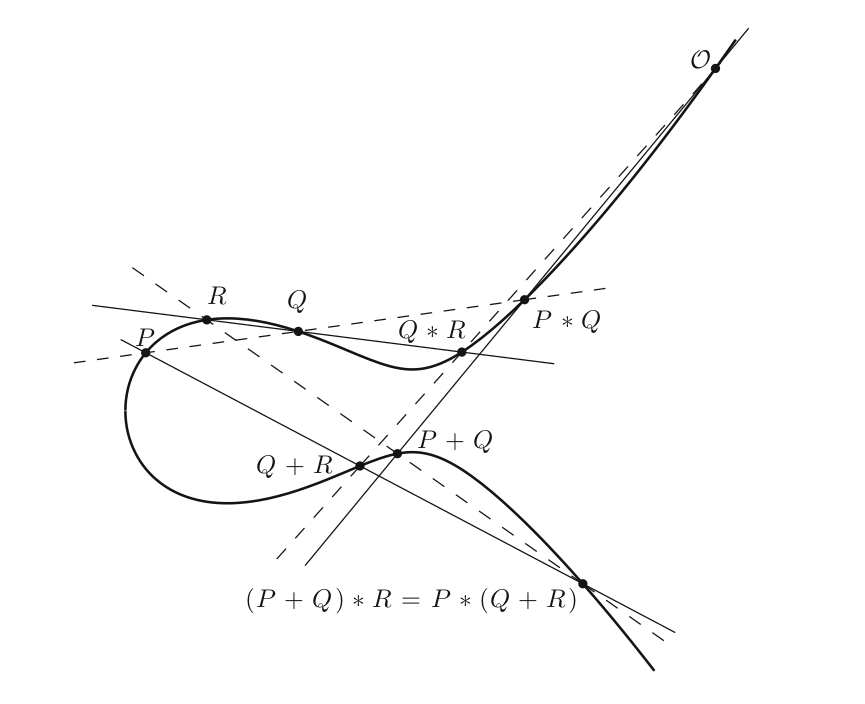
\includegraphics[scale=0.5]{EC4}
\caption{The proof of associatvity of the geometric group law illustrated over the \textit{real} points of an elliptic curve.}
\end{center}
\end{figure}
The union of three lines is a cubic curve since its defining equation is the product of three linear equations. Call $C_1$ the union of the solid lines and $C_2$ the union of the dashed lines. Then, these eight points lie in the intersection of $C_1$, $C_2$, and $E$. Therefore, $N$, the final nineth intersection point of $C_1$ and $C_2$, must also lie on $E$ proving associativity. 
\end{proof}

\begin{proposition}
The geometric group law is given by rational functions in the coordinates which makes it a regular map in the algebraic geometry sense. This group law makes the elliptic curve into an abelian variety. 
\end{proposition}

\begin{proof}
Suppose we want to add points $P, Q \in E$. Let these points have coordinates $P = (x_1, y_1)$ and $Q = (x_2, y_2)$. We will also write $P * Q = (x_3, y_3)$. Then the line between them has the equation,
\[ y = \lambda x + \nu \quad  \lambda = \frac{y_2 - y_1}{x_2 - x_1} \quad \nu = y_1 - \lambda x_1 = y_2 - \lambda x_2 \]
We need to intersect this with $E$ which is defined by,
\[ y^2 = x^3 + a x + b \]
Therefore we need to solve,
\[ (\lambda x + \nu)^2 = x^3 + a x + b \]
which gives,
\[ x^3 - \lambda^2 x^2 + (a - 2 \lambda \nu) x + b - \nu^2 = 0 \]
We know that $x_1$ and $x_2$ are solutions to this since they both line on the line at the elliptic curve. Therefore we can factor,
\[  x^3 - \lambda^2 x^2 + (a - 2 \lambda \nu) x + b - \nu^2 = (x - x_1)(x - x_2)(x - x_3) \]
Therefore, matching $x^2$ coefficients,
\[ \lambda^2 = x_1 + x_2 + x_3 \]
which implies that,
\[ x_3 = \left( \frac{y_2 - y_1}{x_2 - x_1} \right)^2 - x_1 - x_2 \quad \text{and} \quad y_3 = \lambda x_3 + \nu = \left( \frac{y_2 - y_1}{x_2 - x_1} \right)^3 - (2x_1 + x_2) \left( \frac{y_2 - y_1}{x_2 - x_1} \right) + y_1  \]
These are clearly rational functions in the coordinates. There are special cases to consider, for example when $P = Q$ and we must take the tanget line or the line $PQ$ is vertical so $\lambda$ is undefined but all these cases are straigtforward and will give rational functions. 
\end{proof}

\begin{proposition}
The geometric group law and the analytic group law coincide.
\end{proposition}

\begin{proof}
Let $\Lambda \subset \C$ be a lattice, $E$ the associated elliptic curve over $\C$ and $\Phi_{\wp} : \C / \Lambda \to E$ the map induced by the Wierstrass $\wp$-function. For $P \in E$ let $T_P : E \to E$ be the map $Q \mapsto P + Q$. Then define, $\tau_P = \Phi_{\wp}^{-1} \circ T_P \circ \Phi_{\wp} : \C / \Lambda \to \C / \Lambda$. The map $\tau_P$ is holomorphic because $\Phi_{\wp}$ is biholomorphic and $T_P$ is given by rational functions. Let $\pi : \C \to \C / \Lambda$ be the projection map and take $g = \tau_P \circ \pi$ which is doubly periodic. Then $g' : \C \to \C$ is a well-defined holomorphic function since, although its image is only defined up to addition by $\omega \in \Lambda$, its derivative is invariant under addition by a constant. Thus, $g'$ is holomorphic and doubly periodic so $g'$ is constant. Thus $g$ is a linear function so $\tau_P = c_P z + d_P$ where $c_P$ and $d_P$ are constants determined by $P$. Firstly, 
\[ \tau_P(0) = d_P =  \Phi_{\wp}^{-1} \circ T_P \circ \Phi_{\wp}(0) = \Phi_{\wp}^{-1}(T_P(O)) = \Phi_{\wp}^{-1}(P + O) = \Phi_{\wp}^{-1}(P) \]
Secondly, since $T_A$ is an automorphism of $E$ and $\Phi_{\wp}$ is a bijection, $\tau_P$ is a map of the fundamental domain $D$ onto itself bijectivly which must preserve area so $|c_P| = 1$. If $c_p \neq 1$ then $c_P z + d_P = z$ has a solution, namely $z = d_P (1 - c_P)^{-1}$ so $\tau_P$ has a fixed point. However, if $\tau_P(z) = z$ then 
\[ T_P \circ \Phi_{\wp}(z) = \Phi_{\wp} \circ \tau_P(z) = \Phi_{\wp}(z) \]
so $\Phi_{\wp}(z)$ is a fixed point of $T_P$ i.e. $P + \Phi_{\wp}(z) = \Phi_{\wp}(z)$ which cannot happen unless $P = O$ since $(E, +)$ is a group. However, in the case $P = O$ we have $T_O = \id_E$ so $\tau(z) = z$. Thus, either way, $c_P = 1$ so $\tau_P(z) = z + \Phi_{\wp}^{-1}(P)$. Therefore, the geometric group law action $T_P$ is equivalent to a translation $\tau_P(z) = z + \Phi_{\wp}^{-1}(P)$ on the complex torus. In particular, we defined the analytic group law by,
\[ P +_A Q = \Phi_{\wp}(\Phi_{\wp}^{-1}(P) + \Phi_{\wp}^{-1}(Q)) = \Phi_{\wp} \circ \tau_P \circ \Phi_{\wp}^{-1}(Q) = T_P(Q) = P +_G Q \]
which equals the geometric group law.
\end{proof}

\begin{remark}
Since we assumed almost nothing about the geometric group law in this proof, we actually proved a far more remarkable fact. We proved that there is a \textit{unique} group law on $E$ whose identity is the distinguished point $O$ and which is regular with respect to $\wp$ in the sense that $\Phi_{\wp} \circ T_P \circ \Phi_{\wp}^{-1} : \C / \Lambda \to \C / \Lambda$ is holomorphic. This is true of the geometric group law because it is given by rational functions. This extremely powerful uniqueness shows that there cannot be any other group law on $E$ given by rational functions or even by holomorphic functions in the above sense. Requiring that $T_P$ be a regular map is the defining property of an \textit{algebraic group} or, here in the special case of projective algebraic varieties, of an \textit{abelian variety}. We have shown that the geometry of our elliptic curve determines completely and rigidly the algebraic stucture on it. It is exactly this rigidness which makes the group law on an elliptic curve such a natural and indespensible tool for studying the geometry which uniquely determines it. 
\end{remark}


\section{The Mordell-Weil Theorem}

One of the most supprising and powerful theorems in the theory of elliptic curves (and abelian varieties in general) is the Mordell-Weil theorem. This theorem tells us that the structure group structure of the points on an elliptic curve over a number field is especially simple. The theorem is very powerful and I will give it in generality. However, we will only dicuss the special case for elliptic curves defined over $\Q$.

\begin{theorem}[Mordell-Weil]
Let $A$ be an abelian variety defined over a number field $K$ then $A(K)$ the $K$-points of $A$  form a finitely-generated abelian group.
\end{theorem} 

\begin{theorem}[Mordell] 
The case with $A = E$, an elliptic curve, and $K = \Q$ gives that the rational points on an elliptic curve form a finitely generated abelian group i.e there exists finitely many elements $P_1, \dots, P_k \in E(\Q)$ such that any $Q \in E(\Q)$ can be written in the form,
\[ Q = n_1 P_1 + \cdots + n_k P_k \] 
\end{theorem}

\subsection{The Elementary Theory of Heights}

The proof of Mordell-Weil will use a suprising idea, the height of a number. A height function is a function which measures the ``complexity'' of the coordinates of a point. For the case of rational points $E(\Q)$, a possible choice is,
\[ H(\frac{a}{b}) = \max\{ |a|, |b| \} \]
When written in lowest terms. Furthermore, the hieght of a rational point we will simply take to be the height of the $x$-coordinate. We can construct a similar notion of the height of an algebraic number by measuing the size of the coefficients of the minimal polynomial with integer coefficients that is solves. The fundamental property of a height function is that there are a finite number of points with height less than any fixed bound. This fundamental property will allow us to show that various sets of points are finite given that they have a bounded height. It will be convinient to use the `small height'' defined as $h(P) = \log{H(P)}$. First we will state some lemmata.

\begin{lemma}
For every real number $M$, the set,
\[ \{ P \in E(\Q) \mid h(P) \le M \} \]
is finite.
\end{lemma} 

\begin{lemma}
Let $P_0$ be a fixed rational point of $E$. There exists a constant $\kappa_0$ depending on $P_0$ and $E$ such that,
\[ h(P + P_0) \le 2 h(P) + \kappa_0 \]
for any $P \in E(\Q)$. 
\end{lemma}

\begin{lemma}
There exists a constant $\kappa$ depending only on $E$ such that,
\[ h(2 P ) \ge 4 h(P) - \kappa \]
for all $P \in E(\Q)$. Therefore, doubling a point increases the height significantly. 
\end{lemma}

\begin{lemma}
The quotient group $E(\Q) / 2 E(\Q)$ is finite. That is, there are finitely many cosets of the subgroup $2 E(\Q)$ which is the image of the map $P \mapsto P + P = 2 P$. 
\end{lemma}

\begin{remark}
These lemmata will allow us to prove Mordell-Weil by envoking the following descent theorem. The above relate the height, a fundamentally number theoretic concept, to the geometric group law. We can think of the height as translating geometric information about the curve into number theoretic information.
\end{remark}  

\subsection{The Descent Theorem}

\begin{theorem}[Descent]
Let $\Gamma$ be an abelian group with a function,
\[ h : \Gamma \to \R_{> 0} \]
satisfying the following properties,
\begin{enumerate}
\item For any positive real $M$ the set $\{ P \in \Gamma \mid h(p) \le M \}$ is finite. 
\item For each $P_0 \in \Gamma$ there exits a constant $\kappa_0$ such that,
\[ h(P + P_0) \le 2 h(P) + \kappa_0 \]
for all $P \in \Gamma$.
\item There exists a constant $\kappa$ such that,
\[ h(2 P) \ge 4 h(P) - \kappa \]
for all $P \in \Gamma$.
\end{enumerate}
and furthermore we assume that $\Gamma / 2 \Gamma$ is finite then $\Gamma$ is a finitely generated abelian group. 
\end{theorem}

\begin{proof}
We choose representatives of the finite number of cosets of $2 \Gamma$. Let these be $Q_1, \cdots, Q_n$ such that for any $P$ there always exists some $i_1$ such that,
\[ P - Q_{i_1} \in 2 \Gamma \]
which implies that,
\[ P - Q_{i_1} = 2 P_1 \]
for some $P_1 \in \Gamma$. Now we do the same procedure repeatedly using $P_1$ to get a list,
\begin{align*}
P - Q_{i_1} & = 2 P_1
\\
P_1 - Q_{i_2} & = 2 P_2
\\
& \vdots
\\
P_{m-1} - Q_{i_m} & = 2 P_m
\end{align*}
By substituting each line into the previous we get,
\[ P = Q_{i_1} + 2 Q_{i_2} + 4 Q_{i_3} + \cdots + 2^{m-1} Q_{i_m} + 2^m P_m \]
we are going to show that if we make $m$ large enough than we can make $h(P_m)$ less than some constant which does not depend on $P$. Since there are a finite number of such $P_m$ this will show that any $P$ can be written in terms of a fixed finite set of points. 
\bigskip\\
Applying the second height property with $P_0 = - Q_i$ we get,
\[ h(P - Q_i) \le 2 h(P) + \kappa_i \]
for any $P \in \Gamma$. Since there are finitely many $Q_i$ we may take $\kappa'$ to be the maximum $\kappa_i$. Therefore,
\[ h(P - Q_i) \le 2 h(P) + \kappa \]
for each $Q_i$ and any $P \in \Gamma$. Furthermore, applying the thrid property,
\begin{align*}
4 h(P_j) \le h(2 P_j) + \kappa = h(P_{j-1} - Q_{i_j}) + \kappa \le 2 h(P_{j - 1}) + \kappa' + \kappa 
\end{align*}
We can rewrite this as,
\[ h(P_j) \le \frac{1}{2} h(P_{j-1}) + \frac{\kappa' + \kappa}{4} = \frac{3}{4} h(P_{j-1}) - \frac{1}{4}(h(P_{j-1}) - (\kappa' + \kappa)) \]
From this relation we see that if $h(P_{j-1}) \ge \kappa' + \kappa$ then,
\[ h(P_j) \le \frac{3}{4} h(P_{j-1}) \]
which implies that the sequence of points $P_1, P_2, \dots, P_m$ has decreasing height, at least as fast as the geometic series $\left( \frac{3}{4} \right)^j$, as long as $h(P_j) \ge \kappa' + \kappa$. Since this sequence has zero limit, there must exists an $m$ such that $h(P_j) \le \kappa' + \kappa$ otherwise the sequence will continue to decrease to zero. Therefore, we have shown any any point $P$ can be written as,
\[ P = Q_{i_1} + 2 Q_{i_2} + 4 Q_{i_3} + \cdots + 2^{m-1} Q_{i_m} + 2^m P_m \]
where $P_m$ has height less than $\kappa' + \kappa$. Since there are a finite number of points satisfying this height condition and a finite number of representatives $Q_i$ we can take the finite generating set,
\[ \{ Q_1, Q_2, \dots, Q_n \} \cup \{ R \in \Gamma \mid h(R) \le \kappa' + \kappa \} \]
which we have proven can express any point $P \in \Gamma$ in some finite sum. 
\end{proof}

\begin{remark}
Assuming the lemata, we have proven Mordell's theorem i.e. the special case of Mordell-Weil for elliptic curves and $K = \Q$. To generalize this result requires proving these lemmata, or some appropreate generalization, for the algebraic heigh function over a number field. We will not give the details here. 
\end{remark}


\subsection{The Proof For $K = \Q$}

We will now sketch some of the proofs of the omitted lemmata. (WIP)


\section{The Moduli Space of Complex Tori}

\subsection{Maps Between Complex Tori}

\begin{proposition}
Let $\Lambda, \Lambda \subset \C$ be lattices and $m, b \in \C$ be complex numbers. Then the map, $f : \C / \Lambda \to \C / \Lambda'$ given by $[z] \mapsto [m z + b]$ is a well-defined holomorphic map of complex tori iff $m \Lambda \subset \Lambda'$. 
\end{proposition}

\begin{proof}
Such a map is clearly holomorphic since it is a linear function. We require that it be well-defined i.e. if $z' = z + \omega$ then $f([z']) = f([z])$ since $[z'] = [z]$. Therefore, $[m z + m \omega + b] = [m z + b]$ which is equivalent to $m \omega \in \Lambda'$ for any $\omega \in \Lambda$. This is exactly the condition that $m \Lambda \subset \Lambda'$
\end{proof}

\begin{proposition}
Any holomorphic map $f : \C / \Lambda \to \C / \Lambda'$ must be of the form $[z] \mapsto [m z + b]$ for some complex numbers $m,b \in \C$ such that $m \Lambda \subset \Lambda'$. Furthermore, $f$ is a group homomorphism exactly when $b \in \Lambda'$ i.e. $[b] = 0$ in $\C / \Lambda'$.
\end{proposition}

\begin{proof}
We have seen this argument previously in the connection between the geometric and analytic group law. We will be more careful this time. 
\bigskip\\
Consider the projection maps $\pi : \C \to \C / \Lambda$ then there is a diagram,
\begin{center}
\begin{tikzcd}[column sep = large, row sep = large]
\C \arrow[r, "\tilde{f}", dashed] \arrow[d, "\pi"] & \C \arrow[d, "\pi"]
\\
\C / \Lambda \arrow[r, "f"] & \C / \Lambda' 
\end{tikzcd}
\end{center}
I claim there is a map $\tilde{f} : \C \to \C$ which makes this diagram commute. This is known as lifting to the universal cover in the math lingo but it is easy to see what this map should be. On each parallelogram in $\C$ we want $\tilde{f}$ to just be $f$ up to shifiting by a constant since $\pi \circ \tilde{f} = f \circ \pi$ is defined up to a constant. We glue these together choosing the correct constants to match on the boundaries of the parallelograms.  
\bigskip\\
Now, I claim that $\tilde{f}' : \C \to \C$ is periodic. This is the case because for any $\omega \in \Lambda$ the function, $q_\omega(z) = \tilde{f}(z + \omega) - \tilde{f}(z) \in \Lambda$ since,
\[ \pi \circ q_\omega(z) = \pi \circ \tilde{f}(z + \omega) - \pi \circ \tilde{f}(z) = f([z + \omega]) - f([z]) = f([z]) - f([z]) = 0 \]
But $q_\omega$ is continuous and $\Lambda$ is discrete so $q_\omega$ is constant. Therefore, $q_\omega' = 0$ which implies that $\tilde{f}'(z + \omega) = \tilde{f}'(z)$ so $\tilde{f}'$ is periodic. 
\bigskip\\
Therefore, by Liouville, $\tilde{f}'$ is constant so $\tilde{f} = m z + b$ for some $m,b \in \C$. Therefore, $f([z]) = \pi \circ \tilde{f}(z) = [m z + b]$. Furthermore, we have seen that such a map is well-defined exactly when $m \Lambda \subset \Lambda'$
\bigskip\\
Finally, for $f$ to be a homomorphism we must have $f([z + w]) = f([z]) + f([w])$ and thus,
\[ [m(z + w) + b] = [m z + b] + [m w + b] = [m (z + w) + 2 b] \]
which is equivalent to $[b] = 0$ in $\C / \Lambda'$. 
\end{proof}


\begin{corollary}
The complex tori $\C / \Lambda$ and $\C / \Lambda'$ are isomorphic exactly when there exists a complex number $m \in \C^\times$ such that $m \Lambda = \Lambda'$.
\end{corollary}

\begin{proof}
When this is the case then we have shown there is a holomorphic homomorphism $\C / \Lambda \to \C / \Lambda'$ given by $[z] \mapsto [m z]$. Furthermore, since we have equality, we can invert to find, $\frac{1}{m} \Lambda' = \Lambda$ so we also get a well-defined inverse map $\C / \Lambda' \to \C / \Lambda$ given by $[z] \mapsto [m^{-1} z]$. These homomorphisms are clearly inverse so $\C / \Lambda \cong \C / \Lambda'$.
\bigskip\\
Furthermore, we have shown that any isomorphisms must be of this type so $\C / \Lambda \cong \C / \Lambda'$ implies that $m \Lambda = \Lambda'$ for some $m \in \C^\times$ given by the isomorphism. 
\end{proof}

\begin{remark}
We have reduced classifying complex tori up to isomorphism to a problem of algebra: classifying lattices in $\C$ up to scaling by a complex number. We now turn our attention to studying such lattices.
\end{remark}



\subsection{Lattices}

\begin{remark}
Recall that a lattice $\Lambda \subset \C$ is given by sums of two independent periods $\omega_1, \omega_2 \in \C$ explicitly,
\[ \Lambda = \{ n \omega_1 + m \omega_2 \mid n,m \in \Z \} \]
We first what to know when do periods define the same lattice. First we will fix an orientation.
\end{remark}


\begin{definition}
Let $\h \subset \C$ be the upper half plane,
\[ \h = \{ z \in \C \mid \Im{z} > 0 \} = \{ x + iy \mid x, y \in \R \text{ and } y > 0 \} \]
\end{definition}

\begin{remark}
We say a basis $( \omega_1, \omega_2 )$ of a lattice $\Lambda$ is positively oriented if $\frac{\omega_1}{\omega_2} \in \h$. Notice that if our basis is not positively oriented then we can simply swap the order to get a positively oriented bais. For simplicity, we will only work with such bases from now on. 
\end{remark}

\begin{remark}
For any complex torus $\C / \Lambda$ we can always put our lattices in a standard form, 
\[ \Lambda_\tau = \{ n \tau + m \mid n,m \in \Z \} \]
for some $\tau \in \h$. To see this choose a positively oriented basis $(\omega_1, \omega_2)$ for $\Lambda$ and then,
\[ \frac{1}{\omega_2} \Lambda = \{ \tfrac{\omega_1}{\omega_2} n + m \mid n, m \in \Z \}  = \Lambda_{\tau} \]
where $\tau = \frac{\omega_1}{\omega_2} \in \h$ by the positive ordering. Furthermore, there is a unique lattice up to scaling in standard form since to preserve the basis element $1$ the scaling must be trivial. This argument shows that there is a unique lattice in standard form for each isomorphism class of complex tori since isomorphisms of complex tori are given by scaling their lattices. 
\end{remark}

\begin{definition}
The modular group $\MG$ is defined the group of matrices with integer coefficients and determinant one,
\[ \MG = \left\{ \begin{pmatrix}
a & b 
\\
c & d
\end{pmatrix} \quad \middle| \quad a,b,c,d \in \Z \text{ and } ad - bc = 1  \right\} \]
\end{definition}

\begin{proposition}
Positively oriented bases $(\omega_1, \omega_2)$ and $(\omega_1', \omega_2')$ generate the same lattice $\Lambda$ iff,
\[ \begin{pmatrix}
\omega_1'
\\
\omega_2' 
\end{pmatrix}
=
\begin{pmatrix}
a & b 
\\
c & d
\end{pmatrix}
 \begin{pmatrix}
\omega_1
\\
\omega_2
\end{pmatrix} \]
for some matrix,
\[ \begin{pmatrix}
a & b 
\\
c & d
\end{pmatrix} \in \MG \]
\end{proposition}

\begin{proof}
Let $(\omega_1', \omega'_2)$ and $(\omega_1, \omega_2)$ generate $\Lambda'$ and $\Lambda$. Suppose that $\Lambda' \subset \Lambda$ then $\omega'_1, \omega_2' \in \Lambda$ so we must have,
\begin{align*}
\omega_1' & = a \omega_1 + b \omega_2
\\
\omega_2' & = c \omega_1 + d \omega_2 
\end{align*}
However, if $\Lambda' = \Lambda$ then $\Lambda \subset \Lambda'$ so there exist integers satisfying the inverse relation. Thus,
\[ \gamma = \begin{pmatrix}
a & b 
\\
c & d
\end{pmatrix} \] 
has an integer inverse i.e. $\gamma \in \GL{2}{\Z}$. It suffices to show that $\det{\gamma} = 1$. Since $\gamma \in \GL{2}{\Z}$ we know that $\det{\gamma} = \pm 1$ since the determinant must have a multiplicative inverse in $\Z$. The condition that both bases are positivly oriented means that $\det{\gamma} > 0$ proving the proposition. 
\end{proof}

\begin{remark}
Consider how this proposition works on lattices $\Lambda_{\tau}$ in standard form. It says that we can act on the basis $(\tau, 1)$ by some matrix,
\[ \gamma = \begin{pmatrix}
a & b 
\\
c & d
\end{pmatrix} \in \MG \]
to get,
\[ \begin{pmatrix}
a & b 
\\
c & d
\end{pmatrix}
 \begin{pmatrix}
\omega_1
\\
\omega_2
\end{pmatrix}
= \begin{pmatrix}
a \tau + b 
\\
c \tau + d
\end{pmatrix} \]
so $\Lambda_{\tau} = \{ (a \tau + b) n + (c \tau + d) \mid n, m \in \Z \}$. We can put this lattice in standard form by the usual trick to get,
\[ \Lambda_{\tau'} = \frac{1}{c \tau + d} \Lambda_{\tau} \]
where,
\[ \tau' = \frac{a \tau + b}{c \tau + d} \]
Therefore, doing this strange matrix transformation to $\tau$ does not change the corresponding complex torus. 
Accordingly, we define an action of $\MG$ on points $\tau \in \h$ via,
\[ \gamma \cdot \tau = \frac{a \tau + b}{c \tau + d} \]
We can check that $\tau' \in \h$ and that $(\gamma_1 \gamma_2) \cdot \tau = \gamma_1 \cdot (\gamma_2 \cdot \tau)$. 
Also, since every lattice has a unique standard form and lattices are equivalent exactly when they linked by some $\MG$ action and complex tori are isomorphic exacly when their corresponding lattices are equal up to scaling we have shown that there is a unique isomorphism class for each $\tau \in \h$ up to the action of $\MG$.
\end{remark} 

\begin{theorem}
Consider the space $\mathfrak{M} = \h / \MG$ which are orbits of $\tau \in \h$ under the action of $\MG$. There is a unique isomorphism class of complex tori for each $\tau \in \mathfrak{M}$ represented by $\C / \Lambda_\tau$. We therefore call $\mathfrak{M}$ the \textit{moduli space} of complex tori. 
\end{theorem}

\begin{remark}
The modular group is extremely important in what follows so it is vital to understand its properties. 
\end{remark}

\begin{proposition}
$\MG$ is generated by the two matrices,
\[ \begin{pmatrix}
1 & 1 
\\
0 & 1
\end{pmatrix}
\quad \quad \quad
\begin{pmatrix}
0 & -1 
\\
1 & 0
\end{pmatrix} \]
These correspond to the transformations of lattices $\tau \mapsto \tau + 1$ and $\tau \mapsto - \frac{1}{\tau}$. 
\end{proposition}  

{\color{red} (DRAW THESE CORRESPONDING LATTICE TRANS) }


\section{Modular Forms}

\subsection{Discriminants}

\begin{remark}
For a quadratic equation, 
\[ a x^2 + b x + c \]
we all know that the roots are given by,
\[ \alpha_{\pm} = \frac{-b \pm \sqrt{b^2 - 4 ac}}{2 a} \]
Notice that the quantity,
\[ \Delta = b^2 - 4 ac \]
determines the number and reality of the roots. We call this quantity the discriminant. We would like to look for an analogous quantity for higher-order polynomials. Notice that,
\[ \Delta = (\alpha_{+} - \alpha_{-})^2 \]
\end{remark}

\begin{definition}
Given a polynomial $f(z) \in \C[z]$ of degree $n$, we know that $f$ has exactly $n$ roots $\alpha \in \C$ (counted with multiplicity). We define the \textit{discriminat} of $f$ to be,
\[ \Delta(f) = \prod_{i < j} (\alpha_i - \alpha_j)^2 \]
Notice that $f(z)$ has a double root iff $\Delta(f) = 0$.
\end{definition}

\begin{proposition}
The discriminat $\Delta(f)$ can be written as a polynomial in the coefficients of $f(z)$.
\end{proposition}

\begin{remark}
We have already seen how for a quadratic $f(z) = a z^2 + b z + c$ then $\Delta(f) = b^2 - 4 a c$ is a polynomial in the coefficients of $f$. Now we see how we can do this for a cubic which will be the main case we care about.
\end{remark}

\begin{proposition}
For a cubic of the form $x^3 + p x + q$ we have,
\[ \Delta = - 4 p^3 - 27 q^2 \]
\end{proposition}

\begin{proof}
Recall that a monic polynomial is determined exactly as,
\[ f(x) = \prod_{i = 1}^n (x - \alpha_i) \]
For the cubic case we have,
\begin{align*}
x^3 + p x + q & = (x -  \alpha_1)(x - \alpha_2)(x - \alpha_3) 
\\
& = x^3 - (\alpha_1 + \alpha_2 + \alpha_3) x^2 + (\alpha_1 \alpha_2 + \alpha_2 \alpha_3 + \alpha_1 \alpha_3) x - \alpha_1 \alpha_2 \alpha_3 
\end{align*}
Therefore we must have,
\begin{align*}
\alpha_1 + \alpha_2 + \alpha_3 & = 0
\\
\alpha_1 \alpha_2 + \alpha_2 \alpha_3 + \alpha_1 \alpha_3 & = p
\\
-\alpha_1 \alpha_2 \alpha_3 & = q
\end{align*}
Now consider,
\begin{align*}
\Delta & = (\alpha_1 - \alpha_2)^2 (\alpha_2 - \alpha_3)^2 (\alpha_1 - \alpha_2)^2
\end{align*}
One can show, by expanding out both sides (I don't recommend it) that,
\begin{align*}
\Delta & = - 27 (\alpha_1 \alpha_2 \alpha_3)^2 - 4 \alpha_1 \alpha_2 \alpha_3 (\alpha_1 + \alpha_2 + \alpha_3)^3 + 18 \alpha_1 \alpha_2 \alpha_3 (\alpha_1 + \alpha_2 + \alpha_3)(\alpha_1 \alpha_2  + \alpha_1 \alpha_3 + \alpha_2 \alpha_3) 
\\
& + (\alpha_1 + \alpha_2 + \alpha_2)^2 (\alpha_1 \alpha_2 + \alpha_1 \alpha_3 + \alpha_2 \alpha_3)^2 - 4 (\alpha_1 \alpha_2 + \alpha_1 \alpha_3 + \alpha_2 \alpha_3)^3
\end{align*}
Each factor is a term we know in terms of coefficients so plugging in,
\[ \Delta = - 27 q^2 - 4 p^3 \]
\end{proof}

\begin{remark}
You may wonder how in the hell I knew to write down that expansion of $\Delta$ in terms of the known polynomials. Well it turns out there is general theory which gives an algorithm to do this in general. What do I mean by this? We say a polynomial is symmetric if it remains unchanged under permuting its variables so $\Delta$ is symmetric in the roots $\alpha_i$ and the coefficient polynomials,
\begin{align*}
\alpha_1 + \alpha_2 + \alpha_3
\\
\alpha_1 \alpha_2 + \alpha_2 \alpha_3 + \alpha_1 \alpha_3
\\
\alpha_1 \alpha_2 \alpha_3
\end{align*}
are also symmetric. In fact, these are very special they are called the elementary symmetric polynomials on three variables (think about how you would generalize these to any number of variables). A marvelous theorem says that \textit{any} symmetric polynomial can be decomposed into sums and products of these elementary symmetric polynomials. Furthermore, Vieta's formula tells us that the coefficients of a polynomial are always elementary symmetric polynomials of the roots. Can you see how this proves that the discriminant $\Delta(f)$ must always be some polynomial in the coefficients of $f$ rather than the roots themselves?  Furthermore, the Newton identities actually give an algorithm for computing these expansions in terms of elementary symmetric polynomials. I highly recommend you look into this story further, symmetric polynomials, Newton sum and Newton identities, and Vieta's formula are all good places to start.  
\end{remark}

\begin{remark}
For an elliptic curve defined by a Weirstrass equation,
\[ y^2 = x^3 + a x + b \]
it is important to know when $f(x) = x^3 + a x + b$ has a double root. Why? Consider,
\[ y^2 = (x - \alpha_1)(x - \alpha_2)(x - \alpha_3) \]
and suppose that $\alpha_1 = \alpha_2$. Then there are two solutions,
\[ y = \pm (x - \alpha_1) \sqrt{x - \alpha_3} \]
However note that if $x > \alpha_3$ then close to $(\alpha_1, 0)$ the solutions look like two crossed lines intersecting at $(\alpha_1, 0)$. This is called a node on a curve and it means the curve is \textit{singular} and thus is not \textit{smooth}. There are lots of nice algebraic geometric properties that the curve loses when it is not smooth so we want to avoid this case. 
\bigskip\\
In this case being smooth is equivalent to requiring that $f(x)$ and $f'(x) = 3 x^2 + a$ have no common zeros and recall that this is exactly the condition for a polynomial to have no repeated roots (if $f$ has a double root then $f(x) = (x - r)^2 q(x)$ so $f(r) = 0$ and $f'(x) = 2 (x - r) q(x) + (x - r)^2 q(x)$ also has $q'(r) = 0$). Furthermore, recall that we constructed the discriminant $\Delta(f)$ in such a way that it is zero exactly when $f$ has repeated roots. Therefore, our elliptic curve is smooth exactly when,
\[ \Delta(f) = - 4 a^3 - 27 b^2 \neq 0 \]
\end{remark}

\begin{definition}
Consider the lattice $\Lambda_\tau$. Recall the defining equation of the elliptic Weierstrass $\wp$-function defined on $\Lambda_\tau$ is,
\[ y^2 = f(x) = x^3 - (g_2(\tau)/4) x - (g_3(\tau)/4) \]
such that $(\wp(z), \wp'(z)/2)$ satisfy $y^2 = f(z)$,
\[ (\wp'(z)/2)^2  = \wp(z)^3 - (g_2(\tau)/4) \wp(z) - (g_3(\tau)/4) \]
Thus we define the Modular discriminant to be (up to a constant to remove tedious fractions) the discriminant of this cubic,
\[ \Delta(\tau) = - 4^2 \Delta(f) =  g_2(\tau)^3 - 27  g_3(\tau)^2 \]
\end{definition}

\begin{remark}
For $\tau \in \h$ we know that $\C / \Lambda_\tau$ is a smooth torus (unless $\tau \in \R$ in which case the lattice is degenerate which is why we restric to $\Im{\tau} > 0$ strictly). Therefore due to the isomorphism $\C / \Lambda \to E$ the elliptic curve $E$ must also be smooth so $\Delta(\tau) \neq 0$. Thus we have shown that $\Delta(\tau)$ is nonvanishing on $\h$ but must vanish when $\tau \in \R$. However, we have shown how multiple values of $\tau$ can define the same complex torus and thus elliptic curve, those related by modular transformations. We would like a numerical invariant of the curve which does not depend on the choice of $\tau$. The discriminant $\Delta$ is a natural hope but this turns out not to work. To see why we need to consider the transformation of the Eisenstein series which will lead us to modular forms. 
\end{remark}

\subsection{Eisenstein Series}

\begin{remark}
Much earlier, we saw the Eisenstein series $G_k(\Lambda)$ arrise in the defining equation of the Weirstrass $\wp$-function. We defined these series for a given lattice but we now know that we can do a modular transformation to our lattice which leaving the complex torus in question invariant. Therefore, we should investigate how our defining equation and thus the Eisenstein series change under a modular transformation.  
\end{remark}

\begin{definition}
For a lattice $\Lambda \subset \C$ we define the Eisenstein series,
\[ G_k(\Lambda) = \sum_{\omega \in \Lambda^\times} \frac{1}{\omega^{2k}} \]
Explicitly, for the lattice $\Lambda = \{ n \omega_1 + m \omega_2 \mid n,m \in \Z \}$ with periods $\omega_1, \omega_2$ we have,
\[ G_k(\Lambda) = \sum_{n,m \neq 0} \frac{1}{(n \omega_1 + m \omega_2)^{2k}} \]
In particular, for the lattice $\Lambda_{\tau}$ in normal form we have,
\[ G_k(\tau) = \sum_{n,m \neq 0} \frac{1}{(n \tau + m)^{2k}} \]
where we now view $G_k : \h \to \C$ as a function on the upper half plane $\h$. 
\end{definition}

\begin{remark}
We now investigate how $G_k(\tau)$ changes under modular transformations. Consider,
\begin{align*}
G_k(\gamma \cdot \tau) & = \sum_{n,m \neq 0} \frac{1}{(n \gamma \cdot \tau + m)^{2k}} 
\\
& = \sum_{n,m \neq 0} \frac{1}{(n \left( \frac{a \tau + b}{c \tau + d} \right) + m)^{2k}} 
\\
& = (c \tau + d)^{2k} \sum_{n,m \neq 0} \frac{1}{(n (a \tau + b) + m (c \tau + d))^{2k}} 
\\
& = (c \tau + d)^{2k} \sum_{n,m \neq 0} \frac{1}{((an + cm) \tau + (bn + dm)  )^{2k}} 
\end{align*}
Notice that this is the same sum but with basis changed to,
\begin{align*}
\begin{pmatrix}
n'
\\
m'
\end{pmatrix}
=
\begin{pmatrix}
a & c
\\
b & d 
\end{pmatrix}
\begin{pmatrix}
n
\\
m
\end{pmatrix}
= \gamma^{\top} 
\begin{pmatrix}
n
\\
m
\end{pmatrix}
\end{align*}
Recall that since $\gamma^\top \in \MG$ it acts on bases of integral lattices to give equivalent bases. Therefore, $n',m' \in \Z$ range over the same values as $n$ and $m$ meaning that,
\[ G_k(\gamma \cdot \tau) = (c \tau + d)^{2k} \sum_{n',m' \neq 0} \frac{1}{(n' \tau + m')^{2k}} = (c \tau + d)^{2k} G_k(\tau) \]
Therefore, $G_k$ is almost invariant under the action of $\MG$ except for this strange factor of $(c \tau + d)^{-2k}$ in the front. We call this transformation property being weakly modular of weight $2k$ and such a function (with certain regularity conditions) a modular form of weight $2k$.
\end{remark}

\begin{definition}
A meromorphic function $f : \h \to \C$ is weakly modular of weight $k$ if for any $\gamma \in \MG$ we have,
\[ f(\gamma \cdot \tau) = (c \tau + d)^k f(\tau) \]
for all $\tau \in \h$. Note that because $\MG$ is generated by the matrices,
\[ \begin{pmatrix}
1 & 1 
\\
0 & 1
\end{pmatrix}
\quad \quad \quad
\begin{pmatrix}
0 & -1 
\\
1 & 0
\end{pmatrix} \]
which have corresponding actions $\tau \mapsto \tau + 1$ and $\tau \mapsto - \frac{1}{\tau}$ it suffices to check that,
\[ f(\tau + 1) = f(\tau) \quad \text{and} \quad f\left( - \tfrac{1}{\tau} \right) = \tau^k f(\tau) \]
\end{definition}

\begin{definition}
A function $f : \h \to \C$ is a \textit{modular form} of weight $k$ if,
\begin{enumerate}
\item $f$ is holomorphic on $\h$
\item $f$ is weakly modular of weight $k$ i.e. $f(\gamma \cdot \tau) = (c \tau + d)^k f(\tau)$
\item $f$ is holomorphic at $\infty$
\end{enumerate}
\end{definition} 

\begin{remark}
The last property requires some additional explination which we now give. Notice that as $\tau \to i \infty$ the \textit{nome} $q = e^{2 \pi i \tau} \to 0$ since for $\tau = x + i t$ we have,
\[ q = e^{2 \pi i x} \cdot e^{- 2 \pi t} \xrightarrow{t \to \infty} 0 \]
Therefore, to ask that $f$ be ``holomorphic at $\infty$'' we could that $f$ is holomorphic as a function of $q$. But how is $f$ a function of $q$? Consider the function,
\[ g(q) = f \left( \frac{\log{q}}{2 \pi i} \right) \]
then $g(q) = f(\tau)$ for $q = e^{2 \pi i \tau}$. However, the logarithm is not well-defined for complex numbers since $e^{z + 2 \pi i n} = e^z$ for $n \in \Z$. Therefore, $\log{q}$ is multi-valued, its value is only determined up to an element of $2 \pi i \Z$. In fact, we can define $\log : \C^\times \to \C / (2 \pi i \Z)$. However, modularity here steps in to save the day. Recall that $\tau \mapsto \tau + 1$ is the modular transformation for,
\[ \gamma = 
\begin{pmatrix}
1 & 1 
\\
0 & 1
\end{pmatrix} \]
then weak moularity fo $f$ implies that,
\[ f(\tau + 1) = f(\gamma \cdot \tau) = (c \tau + d)^k f(\tau) = f(\tau) \]
Thus, $f$ is periodic by integer steps along the real axis. This solves the multivaluedness issue since,
\[ f \left( \frac{\log{q}}{2 \pi i} \right) \]
is well-defined since it is invariant under $\log{q} \mapsto \log{q} + 2 \pi i n$. 
\bigskip\\
Thus, since $f : \h \to \C$ is holomorphic on all of $\h$ this implies that $g$ is holomorphic on the puntured disc $D^\times = \{ z \in \C^\times \mid |z| < 1 \}$ which is the image of $q = e^{2 \pi i \tau}$ for all $\tau \in \h$. Therefore, $g$ must have a Laurent series at $q = 0$,
\[ g(q) = \sum_{n \in \Z} a_n(f) \: q^n \]
Since $g(q) = f(\tau)$ for $q = e^{2 \pi i \tau}$ we will schematicall write,
\[ f(\tau) = \sum_{n \in \Z} a_n(f) \: q^n \quad \quad q = e^{2 \pi i \tau} \]
which we call the Fourier expansion of $f$. 
\bigskip\\
Finally, we say that $f$ is holomorphic at $\infty$ if $g$ is holomorphic on the entire disc $D$, in particular, if $g$ is holomorphic at $q = 0$. This is equivalent to having no negative terms (poles) in the Laurent series so,
\[ g(q) = \sum_{n = 0}^\infty a_n(f) \: q^n \] 
\end{remark}


(Q-EXPANSION, HOL AT INFINITY, CUSP FORM)

(SPACES OF MODULAR AND CUSPFORMS AND RINGS)

\begin{definition}
A function $f: \h \to \C$ is holomorphic at $\infty$ if $f$ has a Fourier expansion 
\[ f(\tau) = \sum_{n = 0}^{\infty} a_n(f) \: q^n \quad \quad  q = e^{2\pi i \tau} \]
\end{definition}


\begin{remark}
To show a weakly modular holomorphic function $f$ is holomorphic at $\infty$ one only needs to show that $f(\tau)$ is bounded as $\Imt(\tau) \to \infty$.
\end{remark}

\begin{definition}
A modular form $f : \h \to \C$ is a \textit{cusp} form if $f$ vanishes at $\infty$ meaning that $a_0(f) = 0$ in its Fourier series. That is,
\[ f(\tau) = \sum^\infty_{n = 1} a_n(f) \: q^n = a_1(f) q + a_2(f) q^2 + \cdots \quad \quad q = e^{2 \pi i \tau} \]
so $g$ vaishes at $q = 0$. This is equivalent to the requirement that $\lim\limits_{t \to \infty} f(i t) = 0$. 
\end{definition}


\begin{definition}
We denote the vectorspace of weight $k$ modular forms by $\M{k}(\MG)$ and the subspace of cups forms by $\S{k}(\MG)$. 
\end{definition}

\begin{remark}
In the theory of modular forms one often considers functions which are only required to by weakly modular with respect to special subgroups $\Gamma \subset \MG$ known as congruence subgroups. In that case we would have larger spaces of modular forms $\M{k}(\Gamma)$ and $\S{k}(\Gamma)$. We will not consider such objects here but they are essential in formulating the modularity theorem and the theory of modular curves. 
\end{remark}

\begin{remark}
Since a weakly modular function of weight $0$ satisfies $f(\gamma \cdot \tau) = f(\tau)$ it is invariant under the action of $\MG$. Thus, we may consider weight $0$ modular forms as functions $f : \mathfrak{M} \to \C$ on the moduli space of complex tori. 
\end{remark}

{ \color{red}


(DO EXPANSION OF J-INVARIANT SHOW THAT EVERY ELLIPTIC CURVE COMES FROM COMPLEX TORUS ALL SAY THIS IS CALLED ALGEBRIZING CUZ ITS COOL)

(TRY TO STATE MODULARITY THEOREM AND HOW IT PROVES FLT)

(TRY TO STATE BSD)


\subsection{Computing Fourier Series of the Eisenstein Forms}

Our goal is to expand the functions,
\[ G_{k}(\tau) = \sum_{a,b \neq 0} \frac{1}{(a \tau + b)^{2k}} \]
in terms of the nome $q = e^{2 \pi i \tau}$. Note that we can split up the terms where $n = 0$ to give,
\[ G_{k}(\tau) = \sum_{b \neq 0} \frac{1}{m^{2k}} + \sum_{a \neq 0} \sum_{b \in \Z} \frac{1}{(a \tau + b)^{2k}}  \]
Therefore, it suffices to understand the series,
\[ s_{2k}(\tau) = \sum_{b \in \Z} \frac{1}{(\tau + b)^{2k}} \]
since we have,
\[ G_{k}(\tau) = 2 \zeta(2k) + 2 \sum_{a = 0}^\infty s_{2k}(a \tau) \]
where,
\[ \zeta(s) = \sum_{n = 1}^{\infty} \frac{1}{n^s} \]
is the Riemann zeta function.
It turns out that,
\[ s_{2k}(\tau) = \frac{(2 \pi i)^{2k}}{(2k - 1)!} \sum_{m = 1}^\infty m^{2k - 1} q^m \]
Assuming this and noting that $q_a = e^{2 \pi i a \tau} = (e^{2 \pi i \tau})^a = q^a$ we then find that,
\[ G_{k}(\tau) = 2 \zeta(2 k) + \frac{2 (2 \pi i)^{2k}}{(2 k - 1)!} \sum_{a = 1}^{\infty} \sum_{m = 1}^{\infty} m^{2k - 1} q^{am} \]
We can rearange these sums by summing over $n = am$ and all possible divisors $m \divides n$,
\[ G_{k}(\tau) = 2 \zeta(2 k) + \frac{2 (2 \pi i)^{2k}}{(2 k - 1)!} \sum_{n = 1}^{\infty} \left( \sum_{m \divides n} b^{2k - 1} \right) q^n \]
These coefficients are called the divisor sum functions for obvious reasons,
\[ \sigma_{r}(n) = \sum_{m \divides n} m^r \]
where $\sigma_0(n)$ is the number of divisors of $n$ and $\sigma_1(n)$ is the sum of the divisors of $n$. Therefore, we have shown that,
\[ G_{k}(\tau) = 2 \zeta(2 k) + \frac{2 (2 \pi i)^{2k}}{(2 k - 1)!} \sum_{n = 1}^{\infty} \sigma_{2k - 1}(n) \: q^n \]
In particular, we need the cases $k = 2$ and $k = 3$ so we need the values of the Riemann zeta function,
\[ \zeta(4) = \frac{\pi^4}{90} \quad \quad \quad \zeta(6) = \frac{\pi^6}{945} \]
these are marvelous facts which we do not have time to prove. I highly encourage you to look up proofs of these facts. Therefore we have,
\begin{align*}
G_2(\tau) & = \frac{\pi^4}{45} + \frac{(2 \pi)^4}{3} \sum_{n = 1}^{\infty} \sigma_{3}(n) \:  q^n = \frac{\pi^4}{45} \left( 1 + 240 \sum_{n = 1}^{\infty} \sigma_{3}(n) \:  q^n\right) = \frac{\pi^4}{45} \left( 1 + 240 q + 2160 q^2 + \cdots \right)
\\
G_3(\tau) & = \frac{2 \pi^6}{945} - \frac{(2 \pi)^6}{60} \sum_{n = 1}^{\infty} \sigma_{5}(n) \: q^n = \frac{2\pi^6}{945} \left( 1 - 504 \sum_{n = 1}^{\infty} \sigma_5(n) \: q^n \right) = \frac{2\pi^6}{945} \left( 1 - 504 q - 16632 q^2 + \cdots\right)
\end{align*} 
Since these series are well-defined at $q = 0$ the Eisenstein series do indeed define modular forms of weight $2k$. 

\subsection{The $j$-invariant of an Elliptic Curve}

We now return to our quest of finding an numerical invariant of complex tori. The modular discriminant $\Delta(\tau)$ turns out not to work because it is not invariant under the modular group. Instead we have the following.

\begin{proposition}
The modular discriminant $\Delta$ is a weight $12$ cusp form i.e. $\Delta \in \S{12}(\MG)$. 
\end{proposition}

\begin{proof}
$\Delta(\tau) = g_2(\tau)^3 - 27 g_3(\tau)^2$ and since $g_2$ has weight $4$ and $g_3$ has weight $6$ both terms have weight $12$. Now we need to consider the $q$-expansion of $\Delta$. Recall that $g_2(\tau) = 60 G_2(\tau)$ and $g_3(\tau) = 140 G_3(\tau)$. Now we use the $q$-expansions of these functions we computed earlier to find,
\begin{align*}
g_2(\tau)^3 & = \frac{4^3 \pi^{12}}{3^3} \left(1 + 720 q + \cdots \right)
\\
27 g_3(\tau)^2 & = \frac{4^3 \pi^{12}}{3^3} \left(1 - 1008 q  + \cdots \right)
\end{align*}
Therefore,
\[ \Delta(\tau) = (2 \pi)^{12} q + O(q^2) \]
Therefore, $\Delta(\tau)$ is holomorphic at infinity and moreover since the constant zero in its $q$-expansion is zero $\Delta$ is a cusp form. 
\end{proof}

\begin{remark}
Therefore under the modular transformation $\Delta(\gamma \cdot \tau) = (c \tau + d)^{12} \Delta(\tau)$ so it is not a good invariant. However, we have annother weight $12$ form so we can take the quotient.
\end{remark}

\begin{definition}
The $j$-invariant $j : \h \to \C$ is a weakly-modular function of weight $0$ (invariant under the modular group) defined as,
\[ j(\tau) = (12)^3 \: \frac{g_2(\tau)^3}{\Delta(\tau)} \] 
\end{definition}

\begin{remark}
This is modular invariant because,
\[ j(\gamma \cdot \tau) = (12)^3 \: \frac{g_2(\gamma \cdot \tau)^3}{\Delta(\gamma \cdot \tau)} = (12)^3 \: \frac{(c \tau + d)^{12} \: g_2(\tau)^3}{(c \tau + d)^{12} \Delta(\tau)} = (12)^3 \: \frac{g_2(\tau)^3}{\Delta(\tau)} = j(\tau) \]
The constant $(12)^3$ is choosen such that the leading coefficent of the Fourier expansion is $1$ as we will now demonstrate. 
\end{remark}

\begin{proposition}
The $j$-invariant has a Fourier expansion,
\[ j(\tau) = \frac{1}{q} + 744 + 196884 q + \cdots \]
\end{proposition}

\begin{proof}
First note that the $(12)^3$ simplifies the $q$-expansion of $g_2(\tau)^3$ to giveme
\[ g_2(\tau)^3 = 4^6 \pi^{12} (1 + 720 q + \cdots) = (2 \pi)^{12} (1 + 720 q + \cdots) \]
Therefore, the $q$-expansion for the $j$-invariant becomes,
\[ j(\tau) = \frac{(2 \pi)^{12} (1 + 720 q + \cdots )}{(2 \pi)^{12} q + \cdots} = \frac{1 + 720 q + \cdots}{q + \cdots} = \frac{1}{q} + O(1) \]
Therefore $j$ has a simple pole at $\infty$ with residue $1$. 
\end{proof}

\begin{remark}
The $j$-invariant is not a modular form since it is not holomorphic but rather meromorphic at $\infty$ since it has a simple pole $q^{-1}$ in its $q$-expansion. We call $j$ a modular function of weight zero or sometimes automorphic form of weight zero. 
\end{remark}

\begin{theorem}
The $j$-invariant $j : \mathfrak{M} \to \C$ is surjective.
\end{theorem}

\begin{proof}
From the Fourier expansion, we have computed,
\[ \lim_{t \to \infty} j(i t) = \infty \]
This, along with the modular invariance, applies that $j$ is a proper map (preimage of compact is compact) so its image is closed. Furthermore, $j$ is holomorphic (and nonconstant) so its image is open. Therefore, it is surjective. To see this consider the compactification,
\[ \hat{j} : \hat{\mathfrak{M}} \to \hat{\C} \]us 
The $j$-invariant extends to a a holomorphic function exact because of this limit condition so it is continuous at $\infty$. Then, we get a nonconstant holomorphic map of compact Riemann surfaces which again is open (by open mapping) and closed (by compactness of the image) and thus is surjective. Furthermore, since $\hat{j}(i \infty) = \infty$ we see that $j : \mathfrak{M} \to \C$ must be surjective since $\hat{j}$ hits all of $\C$ and $i \infty$ is not mapped to $\C$.
\end{proof}



\begin{definition}
By analogy to the complex analytic $j$-invariant, given an elliptic curve $E$ defined by the Wierstrass equation,
\[ y^2 = x^3 - (g_2/4) x - (g_3/4) \]
we define the $j$-invariant of the curve to be,
\[ j(E) = (12)^3 \cdot \frac{g_2^3}{4 g_2^2 - 27 g_3^3} \]
\end{definition}

\begin{theorem}
Two elliptic curves $E$ and $E'$ are isomorphic over  $\C$ if and only if $j(E) = j(E')$.
\end{theorem}

\begin{proof}
Let $E$ and $E'$ be defined by Weierstrass equations,
\[ y^2 = x^3 - a x - b \quad \quad y^2 = x^3 - a' x - b' \]
respectively. Then,
\[ j(E) = (12)^3 \cdot \frac{4 a^3}{4 a^3 - 27 b^2} \]
Suppose that $j(E) \neq 0, (12)^3$ then,
\[ \frac{j(E)}{j(E) - (12)^3} = \frac{4 a^3}{27 b^2} \]
Therefore, $j(E) = j(E')$ implies that,
\[ \frac{a^3}{b^2} = \frac{a'^3}{b'^2} \]
Since we are working over the complex numbers we can choose a square root to get the following $\mu \in \C$ s.t.
\[ \mu^2 = \frac{a b'}{a' b} \]
Then, notice,
\[ \mu^4 a = \frac{a^3 b'^2}{a'^2 b^2} = a' \]
and likewise,
\[ \mu^6  b = \frac{a^3 b'^3}{a'^3 b^2} = b' \]
Therefore, we define a map $(x, y) \mapsto (\mu^2 x, \mu^3 y)$. Consider,
\[ (\mu^3 y)^2 - (\mu^2 x)^3 - a' (\mu^2 x) -  b' = (\mu^3 y)^2 - (\mu^2 x)^3 - \mu^4 a (\mu^2 x) - \mu^6 b  = \mu^6 (y^2 - x^3 - a x - b) \] 
Thus, $(x, y) \in E \implies (\mu^2 x, \mu^3 y) \in E'$. This is clearly invertible so it suffices to check that it is a group homomorphism. Since $E$ is a group the bijection $E \to E'$ induces a group structure on $E'$. Recall that, up to choosing an origin, there is a unique group structure on $E'$ so it suffices to show that the map $E \to E'$ preserves the origin (for affine Weierstrass patches this is canonically chosen to be the point at infinity). In terms of projective coordinates, this map sends $[X : Y : Z] \mapsto [\mu^2 X : \mu^3 Y : Z]$ so the point at infinity $[0 : 1 : 0] \mapsto [0 : \mu^3 : 1] = [0 : 1 : 0]$ proving the theorem. In the case $j(E) = j(E') = 0$ then $a = a' = 0$ so choose $\mu^6 b = b'$ and repeat the argument. For $j(E) = j(E') = (12)^3$ then $b = b' = 0$ so choose $\mu^4 a = a'$ and repeat the argument. 
\end{proof}

\begin{theorem}
Two complex tori $\C / \Lambda$ and $\C / \Lambda'$ are isomorphic iff $j(\Lambda) = j(\Lambda')$. In particular $j : \mathfrak{M} \to \C$ is surjective.
\end{theorem}

\begin{proof}
If $\C / \Lambda \cong \C / \Lambda'$ then $j(\Lambda) = j(\Lambda')$ since scalling the lattice does not change $j$ and $j$ is invariant under the modular group whose orbits are isomorphism classes of lattices in standard form. Now suppose that $\C / \Lambda \cong \C / \Lambda'$. The Weierstrass $\wp$-function associates these tori to elliptic curves $\C / \Lambda \cong E$ and $\C / \Lambda' \cong E'$. By definition $j(E) = j(\Lambda)$ and thus $j(E) = j(E')$ so $E \cong E'$ and thus $\C / \Lambda \cong \C / \Lambda'$.  
\end{proof}

\begin{theorem}[Algebrization]
Every elliptic curve over $\C$ comes from Weierstrass elliptic functions. Furthermore every complex torus is algebrizable.  
\end{theorem}

\begin{proof}
Given an elliptic curve $E$ consider $j(E) \in \C$. Since the $j$-invariant $j : \mathfrak{M} \to \C$ is surjective, there exists $\tau \in \mathfrak{M}$ such that $j(\tau) = j(E)$. Then, the Weierstrass $\wp$-function gives an isomorphism to an elliptic curve, $\C / \Lambda_{\tau} \xrightarrow{\Phi_\wp} E_\wp$ where $j(E_\wp) = j(\Lambda_{\tau}) = j(\tau) = j(E)$. Therefore, by the previous theorem $E \cong E_\wp$ so we get $\C / \Lambda_\tau \cong E$.
\end{proof}


\section{The Modularity Theorem}


We saw that the $j$-invariant could be extended to a function of compact Riemann surfaces $\hat{j} : \hat{\mathfrak{M}} \to \hat{\C}$. In fact, we have shown that $\hat{j}$ is an isomorphism so the moduli space of complex tori is isomorphic to the Riemann sphere. 
\bigskip\\
Recall when I introduced the notion of a modular form  I remarked that we often do not require modular invariance under the full group $\MG$ but rather a ``congruence subgroup'' $\Gamma \subset \MG$. There is a particularly interesting family of such congruence subgroups,
\[ \Gamma_0(N) = \left \{ 
\begin{pmatrix} a & b 
\\
c & d
\end{pmatrix} 
\: \middle| \: a d - b c = 1 \: \: \mod{c}{0}{N}  
\right \} \]
Then we can define a larger moduli space $\mathfrak{M}_0(N) = \h / G_0(N)$. In the same way that $\mathfrak{M}$ parametrized all complex tori, it turns out $\mathfrak{M}_0(N)$ parametrizes complex tori $E$ with a distinguished order $N$ cyclic subgroup $C$ where two such pairs are isomorphic if there is an isomorphism $E \to E'$ restricting to an isomorphism $C \to C'$ of the distinguished subgroups. We then define the modular curve $X_0(N) = \hat{\mathfrak{M}}_0(N)$ as the compactification of this extended moduli space. This alows us to state an analytic form of the modularity theorem relating these modular curves to elliptic curves with rational $j$-invariants.

\begin{theorem}[Modularity]
Let $E$ be a complex elliptic curve with $j(E) \in \Q$. Then for some positive integer $N$ there eixsts a surjective holomorphic map,
\begin{center}
\begin{tikzcd}
X_0(E) \arrow[r] & E
\end{tikzcd}
\end{center}
\end{theorem}

\begin{remark}
The modularity theorem was the missing piece of  the puzzle whose verification alowed Andew Wiles' to prove Fermat's Last Theorem (FLT). Very roughly, the proof proceeds by, for any counter-example to Fermat Last Theorem, constructing a corresponding elliptic curve which cannot come from modular functions in the sense of the modularity theorem. Then Wiles and collaborators were able to prove the modularity theorem as thus establish a proof of FLT. 
\end{remark}


The modulariety theorem says that all rational elliptic curves arise from modular forms. This was suggested by Taniyama in 1950's, and proved by Wiles and Taylor. Finish the prove of Fermat's last theorem.

Let $E$ is an elliptic curve defined by \[y^2 = 4x^3 - g_2x - g_3\] given that $g_2, g_3 \in \Z$ and $g_2^3 - 27 g_3^2 \ne 0$.

Then for each prime number $p$, we define a number $a_p(E)$ associated to this ellptic curve $E$ by 
\[a_p(E) = p - \#\{(x, y) \in (\Z/p\Z)^2: E(x,y) = 0\}.\]

Let modular form be defined as above, with the Fourier expansion 
\[f(\tau) = \sum_{n = 0}^\infty a_n(f) e^{2 \pi i n \tau}, a_n(f) \in \C\;\; \forall n.\]

The modular form of given weight and level form a vector space. There are linear operators called Hecke operator $T_p$, for each prime $p$. An eigenform is a modular form that is a simultaneous eigenvector for all the Hecke operators. The modularity theorem associate to the equation $E$ an eigenform $f = f_E$ in a vector space of weight 2 modular forms at level $N$. The eigenvalues of $f$ are its Fourier coefficients. 
\[T_p(f) = a_p(f)f.\]
The theorem states that the Fourier coefficient gives the solution counts, 
\[a_p(f) = a_p(E)\] for all primes $p$.

We can also phrase this result in term of $L$-series. We can define $L$-function in general as 
\[L(s) = \sum_{n = 1}^\infty \frac{a_n}{n^s},\] if $a_n$ here is $s_n(f)$ for a weight 2 Hecke eigenform of level N, then the $L$-series has the corresponding factorization
\[L(s, f) = \prod_p (1 - a_p(f)p^{-s} 1_N(p)p^{1-2s})^{-1},\]
the product is taken over all the primes $p$, and $1_N(p)$ is 1 if $p \nmid N$, and $0$ otherwise.

We can define the Hasse-Weil $L$-function of an elliptic curve $E$ in term of $a_p(E)$.

}


\begin{remark}
Warning! Advanced material including Galois theory assumed beyond this point. Should not be attempted by the faint of heart! However, the main meat of this course has already been covered the next sections will give a more number theoretical application of elliptic curves to giving explcit constructions of interesting extensions of quadratic number fields. 
\end{remark}

\newcommand{\rd}[1]{{\color{red} #1 }}

\rd{

\section{Complex Multiplication}


\begin{remark}
We will study the endomorphisms of a complex torus $\C / \Lambda$ which is a group homomorphism $\phi : \C / \Lambda \to \C / \Lambda$. Recall that any such map takes the form $z \mapsto \alpha z$ for some $\alpha \in \C$ such that $\alpha \Lambda \subset \Lambda$.
\end{remark}

\begin{definition}
Clearly for any integer $n \in \Z$ the map $z \mapsto n z$ is an endomorphism since $n \Lambda \subset \Lambda$. We say a complex torus $\C / \Lambda$ has \textit{complex multiplication} or CM if there exists an endomorphism $\phi : \C / \Lambda \to \C / \Lambda$ defined by some noninteger complex number $\alpha \in \C$. 
\end{definition}

\begin{example}
For $\tau = i$, the complex torus $\C / \Lambda_\tau$ where $\Lambda_\tau = \{n + i m \mid n,m \in \Z \}$ has complex multiplication. This is because $i \Lambda = \Lambda$ since $i ( n + i m) = - m + i m \in \Lambda$. 
\end{example}

\begin{proposition}
Let $\Lambda_\tau$ have complex multiplication by $\alpha$. Then $\tau$ and $\alpha$ are imaginary quadratics and $\alpha$ is an imaginary quadratic algbraic integer. 
\end{proposition}

\begin{proof}
We know that $\alpha \Lambda \subset \Lambda$ or equivalently $\alpha \cdot \tau = \tau n_1 + m_1$ and $\alpha \cdot 1 = \tau n_2 + m_2$ for integers $n_1, n_2,m_1, m_2 \in \Z$. Therefore,
\[ (\tau n_2 + m_2) \cdot \tau = \tau n_1 + m_ 1 \]
which implies that,
\[ n_2 \tau^2 + (m_2 - n_1) \tau - m_1 = 0 \]
Also, $\tau \in \h$ so $\tau$ is imaginary quadratic. Furthermore,
\[ \tau = \frac{\alpha - m_2}{n_2} \quad \quad \tau (\alpha - n_1) = m_1 \]
and thus,
\[ (\alpha - n_1) \cdot (\alpha - m_2) = m_1 n_2 \]
or expanding,
\[ \alpha^2 - (n_1 + m_2) \alpha + m_1 m_2 - m_1 n_2 \]
and thus $\alpha$ is a quadratic algebraic integer. Furthermore, suppose $\alpha \in \R$ then since $\tau \notin \R$ we must have $\alpha \cdot 1 = m_2$ so $\alpha \in \Z$ which we assume is not the case for $\Lambda_\tau$ to have complex multiplication. Thus $\alpha$ is an imaginary quadratic integer. 
\end{proof}

\newcommand{\ints}[1]{\mathcal{O}_{#1}}
\newcommand{\embed}{\hookrightarrow}

\begin{definition}
Let $\Lambda$ be a lattice then we define a field extension $K_\Lambda = \Q(\{ \alpha \in \C \mid \alpha \Lambda \subset \Lambda \})$.
\end{definition}

\begin{remark}
When $\Lambda$ is not CM then clearly $K_\Lambda = \Q$ since all such $\alpha \in \C$ are integers. 
\end{remark}

\begin{proposition}
Let $\Lambda$ have complex multiplication by $\alpha$ then $K_\Lambda = \Q(\alpha)$.
\end{proposition}

\begin{proof}
Clearly $\Q(\alpha) \subset K_\Lambda$ so it suffices to show the other inclusion namely that any endomorphism of $\C / \Lambda$ is generated by $1$ and $\alpha$ over $\Q$. 
\bigskip\\
We know that $\alpha = \tau n + m$ for some $n, m \in \Z$ so either $n = 0$ in which case $\alpha \in \Q$ or,
\[ \tau = \frac{\alpha - m}{n} \]
in which case $\tau \in \Q(\alpha)$. Then for any other $\alpha' \Lambda \subset \Lambda$ we have $\alpha' = \tau n' + m'$ for $n', m' \in \Z$. Since $\tau \in \Q(\alpha)$ then $\alpha' \in \Q(\alpha)$ proving the proposition. 
\end{proof}

\begin{remark}
In particular, either $K_\Lambda = \Q$ or $K_\Lambda = \Q(\alpha)$ is an imaginary quadratic field which we call a CM-field as per the following definition. 
\end{remark}

\begin{definition}
We say a number field $K$ is a CM-field if it is a quadratic extension $K / F$ where $F$ is totally real i.e. every embedding $F \embed \C$ factors through $\R \embed \C$ (meaning its image is real) but $K$ is totally imaginary i.e. no embedding $F \embed \C$ factors through $\R \embed \C$ (meaning its image is complex). 
\end{definition}

\begin{remark}
Thus $\Lambda$ has CM iff $K_\Lambda$ is a CM-field since $K / \Q$ of degree $ < 4$, is CM exactly when $K$ is imaginary quadratic. 
\end{remark}

\begin{proposition}
Given $\C / \Lambda$ set $K = K_\Lambda$. If $\C$ has complex multiplication by some minimal $\alpha$ then the endomorphism ring of $\C / \Lambda$ is $\End{(\C / \Lambda)} \cong \Z[\alpha] \subset \ints{K}$. 
\end{proposition} 

\begin{proof}
The field $K$ is generated by $\alpha \in \C$ such that $\alpha \Lambda \subset \Lambda$ which are all algebraic integers. Therefore, there is a map $\End{(\C / \Lambda)} \to \ints{K}$ by $\phi_\alpha \mapsto \alpha$. This is clearly an injective ring map whose image is $\Z[\alpha]$ by the previous result.
\end{proof}

\begin{remark}
When $\Lambda$ does not have complex multiplication then $K_\Lambda = \Q$ which has integers $\Z \cong \End{(\Lambda)}$. When $\Lambda$ has complex multiplication by a primitive $\alpha$ then $K_\Lambda = \Q(\alpha)$ and, 
\[ \End{(\C / \Lambda)} = \Z[\alpha] \subset \Q(\alpha) \]
\end{remark}

\begin{theorem}
If $\Lambda$ has CM then $j(\Lambda)$ is an algebraic integer and $[\Q(j(\Lambda)) : \Q] = h_K$ where $h_K$ is the class number of $K_\Lambda$. Furthermore $\Q(j(\Lambda))$ is the Hilbert Class field of the imaginary quadratic extension $\Q(\tau) / \Q$.
\end{theorem}

\begin{proof}
(HARD)
\end{proof}

\begin{theorem}
If $\tau$ is an imaginary quadratic integer number then $\Lambda_\tau$ has complex multiplication.
\end{theorem}

\begin{proof}
Consider $\tau \Lambda_\tau = \{ \tau^2 n + \tau m \mid n, m \in \Z \}$. However, it $\tau$ is a quadratic integer then it satisfies some monic,
\[ \tau^2 = a \tau + b \]
and thus,
\[ \tau \Lambda_\tau = \{  (a n + m) \tau + bn \mid n, m \in \Z \} \subset_{\tau} \]
Therefore $\Lambda_\tau$ has complex multiplication by $\tau$. 
\end{proof}

\begin{definition}
We call $d$ a Heegner number if it is squarefree and $\Q(\sqrt{-d})$ has clas number $1$ or equivalently its ring of integers is a PID.
\end{definition}

\begin{theorem}[Stark-Heegner]
The only Heegner numbers are,
\[ d = 1, 2, 3, 7, 11, 19, 43, 67, 163 \]
\end{theorem}

\begin{remark}
Here, I cannot restrain myself from telling a wonderous story. Ramanujian is famed to have noticed that the transcendental number,
\[ e^{\pi \sqrt{163}} = 640320^3 + 744 - 0.00000000000075\dots \]
is almost exactly an integer. It turns out this is not a coincidence. 
\bigskip\\
Recall that $d = 163$ is a Heegner number and,
\[ \alpha = \frac{1 + \sqrt{-163}}{2} \]
is an algebraic integer. Then, we have shown that the elliptic curve $E = \C / \Lambda_{\alpha}$ has CM and thus $j(E) = j(\alpha)$ is an algebraic integer of degree $h_K$. However, since $\alpha$ is a Heegner number, $h_K = 1$ and thus $j(E)$ is an ordinary rational integer. However, from the $q$-expansion,
\[ j(\alpha) = \frac{1}{q} + 744 + O(q) \]
However, $q = e^{2 \pi i \alpha} = e^{\pi i + \pi i \sqrt{-163}} = - e^{\pi \sqrt{163}}$. However,
\[ \frac{1}{q} + O(q) = j(\alpha) - 744 \in \Z \] 
and thus,
\[ e^{\pi \sqrt{163}} + O(e^{- \pi \sqrt{163}}) \in \Z \]
Therefore, since $e^{- \pi \sqrt{163}}$ is very small, $e^{\pi \sqrt{163}}$ is very close to an integer.
\end{remark}
}

\section{Machinery}

\subsection{Projective Limits}

\begin{definition}
A projective system is a family of objects indexed by a poset $(I, \le)$ with morphisms $f_{ij} : A_j \to A_i$ when $i \le j$ such that,
\begin{enumerate}
\item $f_{ii} = \id_{A_i}$
\item $f_{ik} = f_{ij} \circ f_{jk}$ for all $i \le j \le k$
\item $(I, \le)$ is directed meaning that for every $i, j \in I$ there exists $k \in I$ such that $i \le k$ and $j \le k$. This means that for all $A_i$ and $A_j$ there is an object $A_k$ such that there are maps $f_{ik} : A_k \to A_i$ and $f_{jk} : A_k \to A_j$.
\end{enumerate}
we define the projective limit $\varprojlim A_n$ to be the categorical limit of this system. Concretely, for groups or modules, we can give the explicit construction of such an object,
\[ \varprojlim A_i = \left\{ (a_i)_{I} \in \prod_{i \in I} A_i \: \bigg| \: \forall i \le j : f_{ij}(a_j) = a_{i}  \right\} \]
Therefore, the projective limit is the set of sequences which reduce compatibly under the maps $f$.  
\end{definition}

\noindent
A very important special case is that of a leftward mapping sequence where $I = \N$ with the usual order. 

\begin{definition}
Given a diagram,
\begin{center}
\begin{tikzcd}
A_0 & A_1 \arrow[l, "f_0"'] & A_2 \arrow[l, "f_1"'] & A_3 \arrow[l, "f_2"'] & \cdots \arrow[l, "f_3"']
\end{tikzcd}
\end{center}
we define the projective limit $\varprojlim A_n$ to be the categorical limit of the diagram. Concretely, for groups or modules, we can give the explicit construction of such an object,
\[ \varprojlim A_n = \left\{ (a_n) \in \prod_n A_n \: \bigg| \: \forall n \in \N : f_n(a_n) = a_{n-1}  \right\} \]
Therefore, the projective limit is the set of sequences which reduce compatibly under the maps $f$.  
\end{definition}

\begin{remark}
One should view the projective limit as the object which ``naturally projects'' compatibly with the maps onto each of the given objects. There are clear projection maps $\pi_i : \varprojlim A_n \to A_i$ given by $\pi_i((a_n)) = a_i$. Reversing all the maps, we can define the dual notion called the direct limit which is the objective into which each of the given objects include compatibly via maps $\iota_i : A_i \to \varinjlim A_n$. When the given morphisms are inclusions the direct limit is simply the union. 
\end{remark}

\begin{example}
Let $R$ be a ring. The ring of formal power series on $R$ is
\[ R[[X]] \cong \varprojlim R[X] / X^n R[X] \]
with maps $R[X] / X^{n+1} R[X] \to R[X] / X^n R[X]$ given by reduction modulo $X^n$. The sequences making up the projective limit give the partial sums of a formal power series.
\end{example}

\subsection{Infinite Galois Theory}

\begin{proposition}
Let $F / K$ be Galois. Then there exists an isomorphism,
\[ \Gal{F / K} \cong \varprojlim_{L/K} \Gal{L / K} \] 
where $L$ runs over all finite Galois extensions $K \subset L \subset F$. The projective system is given by the restriction maps $\Gal{L / K} \to \Gal{L' / K}$ when $L' \subset L$. 
\end{proposition}

\begin{proof}
Given $\sigma \in \Gal{F / K}$ we consider the restriction $\sigma |_L$ to each finite Galois extension $L / K$ which are clearly compatible with restrictions between finite extensions. This gives a map to the projective limit. Since each $\alpha \in F$ is algebraic over $K$ we know that $\alpha$ lies in a finite Galois extension of $K$ so if $\sigma$ is trivial on all finite Galois extensions then $\sigma(\alpha) = \alpha$ so $\sigma = \id_F$. Thus the map is injective. Furthermore, an element of the projective limit induces an automorphism of $F / K$ by mapping each $\alpha \in F$ to its image under the automorphism acting on any finite Galois extension containing $\alpha$. Thus the mapping is surjective. 
\end{proof}

\begin{remark}
The above identification gives a natural profinite topology on $\Gal{F/ K}$ by making the projection maps $\Gal{F / K} \to \Gal{L / K}$ continuous for each finite Galois extension $L / K$. In particular, the kernels of these maps $\Gal{F / L}$ are open subgroups and form a neighborhood basis of $\id$. 
\end{remark}

\begin{example}
The absolute Galois group of $\finfield{p}$ is equal to the profinite completion of $\Z$, 
\[ \Gal{\overline{\finfield{p}} / \finfield{p}} \cong \hat{\Z} = \varprojlim \Z / n \Z \]
\end{example}

\begin{theorem}[Galois Correspondence]
Let $F / K$ be a Galois extension with $G = \Gal{F / K}$. There is an inclusion reversing correspondence between \textit{closed} subgroups $H \subset G$ and subfields $K \subset L \subset F$ given by $H \mapsto F^H$ and $L \mapsto \Gal{F / L}$.
Furthermore, finite extensions $K \subset L \subset F$ correspond to open subgroups $\Gal{F / L} \subset G$ whose cosets correspond to embeddings of $L$ into $F$ fixing $K$. Galois extensions $K \subset L \subset F$ correspond to closed normal subgroups. 
\end{theorem}


\subsection{$\ell$-adic Numbers}

\begin{definition}
The $\ell$-adic integers are the projective limit,
\[ \Z_{\ell} = \varprojlim \Z / \ell^n \Z \]
under the maps $\Z / \ell^{n+1} \Z \to \Z / \ell^n \Z$ given by reduction mod $\ell$. 
\end{definition}

\begin{remark}
There is an inclusion $\Z \hookrightarrow \Z_{\ell}$ given by reducing $a \in \Z$ modulo each $\ell^n$. The sequences representing $\Z \subset \Z_{\ell}$ are exactly those which are eventually constant after the largest power dividing the integer in question. Using the intuition gained from the ring of formal power series, we can write any $\ell$-adic integer as a formal ``base-$\ell$'' power series,
\[ z = a_0 + a_1 \ell + a_2 \ell^2 + a_3 \ell^3 + \cdots \]
which is the natural extension of how integers may be represented in base $\ell$. 
Although this expression is simply convenient and suggestive shorthand for the projective limit sequence of partial sums,
\[ z = (a_0, \, a_0 + a_1 \ell, \, a_0 + a_1 \ell + a_2 \ell^2, \, a_0 + a_1 \ell + a_2 \ell^2 + a_3 \ell^3, \, \cdots) \] 
we can actually give meaning to this infinite sum by changing the standard definition of convergence. Define the $\ell$-adic valuation $v_{\ell} : \Z_{\ell} \to \N \cup \{ \infty \}$ by $v_{\ell}((a_i))$ equals the index of the first nonzero term $a_i$ and $v_{\ell}(0) = \infty$. All terms in the sequence past $v_{\ell}((a_i))$ are nonzero because if $a_i = 0$ then $a_{i-1} = f_i(a_i) = 0$. We can then define an absolute value, $|z|_{\ell} = \ell^{-v_{\ell}(z)}$ which gives a non-archimedean metric on $Z_{\ell}$. Under this metric, the sequence of elements in $\Z \subset \Z_{\ell}$ given by these the partial sums
actually does converge to the $\ell$-adic number,
\[ z = a_0 + a_1 \ell + a_2 \ell^2 + a_3 \ell^3 + \cdots \]
because the element,
\[ z - z_{N-1} = z - \sum_{i = 0}^{N-1} a_i \ell^n = a_N \ell^N + a_{N+1} \ell^{N+1} + a_{N+2} \ell^{N+2} + \cdots \]
has valuation $v_\ell(z_n) \ge N$ because $z_N = (0, \cdots, a_N \ell^N, a_{N+1} \ell^{N+1}, \cdots)$ where the first $N-1$ terms are $0$. Therefore, 
\[ |z - z_n|_{\ell} \le \frac{1}{\ell^N} \to 0 \]
so the sequence converges $z_n \to z$.
\end{remark}

\begin{definition}
The $\ell$-adic field is the field of fractions of $\Z_{\ell}$,
\[ \Q_{\ell} = \mathrm{Frac}(\Z_{\ell}) \]
on which we extend the $\ell$-adic valuation to $v_{\ell} : \Q_{\ell} \to \Z$ by $v_{\ell}(a/b) = v_{\ell}(a) - v_{\ell}(b)$. 
\end{definition}

\begin{proposition}
$\Z_{\ell}^\times = \{ z \in \Z_{\ell} \mid |z|_{\ell} = 1 \}$
\end{proposition}

\begin{proof}
Let $z = (a_i) \in \Z_\ell$. If $v_{\ell}(z) > 0$ then $a_0 = 0$ so for any $(b_i) \in \Z_{\ell}$ we have $a_0 b_0 = 0$ so $z \notin \Z_{\ell}$. However, if $v_{\ell}(z) = 0$ then choose $b_n = a_n^{-1} \in \Z / \ell^n \Z$ which exists because $a_n$ is coprime to $\ell$ since it projects down to $a_0 \neq 0$ in $\Z / \ell \Z$. Then we have,
\[ (a_i) \cdot (b_i) = (a_i b_i) = (1) \]
so $z \in \Z_{\ell}^\times$.  
\end{proof}

\begin{proposition}
Every element $z \in \Q_{\ell}$ can be written uniquely as $z = \ell^n u$ where $u \in \Z_{\ell}^\times$ and $n = v_{\ell}(z)$. 
\end{proposition}

\begin{proof}
First we will prove this for $z = (a_i) \in \Z_{\ell}$. Take $n = v_{\ell}(z)$ so we know that $f_{n-1, k}(a_{k}) = 0$ so $\ell^n \divides a_k$ but $\ell^{n+1}$ does not. Thus we can write $a_k = \ell^n u_k$ with $u_k \in (\Z / \ell^k \Z)^\times$. Take $u = (u_k)$ with $u_k = f_{k n}(u_n) \neq 0$ since $\ell \ndivides u_n$ for $k < n$ so clearly $z = \ell^n u$ and $v_{\ell}(u) = 0$. Furthermore, if $z \in \Q_{\ell}$ then $z = \frac{a}{b}$ for $a,b \in \Z_{\ell}$ so we can write $a = \ell^n u$ and $b = \ell^m v$ with $u,v \in \Z^\times$. Thus,
\[ z = \frac{\ell^n u}{\ell^m v} = \ell^{n-m} u v^{-1} \]
with $v_{\ell}(z) = v_{\ell}(a) - v_{\ell}(b) = n - m$ an $u v^{-1} \in \Z_{\ell}^\times$.  
\end{proof}

\begin{proposition}
\[ \Q_{\ell} = \Z_{\ell}\left[ \frac{1}{\ell} \right] = \bigcup_n \frac{1}{\ell^n} \Z_{\ell} \]
Therefore we may represent an element of $\Q_{\ell}$ as a power series,
\[ a_{-N} \ell^{-N} + a_{-N + 1} \ell^{-N + 1} + \cdots + a_0 + a_1 \ell + a_2 \ell^2 + \cdots \]
with only finitely many negative exponent terms.
\end{proposition}

\begin{proof}
By the previous proposition we can write any element $z \in \Q_{\ell}$ as $\ell^{n} u$ for $u \in \Z_{\ell}^\times$ and $n \in \Z$. Therefore, we simply need to invert $\ell$ to get negative powers of $\ell$ to represent all of $\Q_{\ell}$ from $\Z_{\ell}$. 
\end{proof}


\begin{proposition}
$\Z_{\ell}$ is a local PID (and thus a discrete valuation ring) with unique maximal ideal $\ell \Z_{\ell}$ and residue field $\finfield{\ell}$. 
\end{proposition}

\begin{proof}
Let $I \subset \Z_{\ell}$ be an ideal. Consider $n = v_{\ell}(I) = \min \{ v_{\ell}(z) \in \N \mid z \in I \}$ where the minimum value exists by well ordering. Thus, there exists $z_0 \in I$ with $v_{\ell}(z) = n$. I claim that $I = (\ell)^n$. We can write $z_0 = \ell^n u$ for some $u \in \Z_{\ell}^\times$. Therefore, $I \subset (z) = (\ell^n u) = (\ell)^n$. Furthermore for any $z \in I$ we have $v_{\ell}(z) = m \ge n$ so $\ell^n \divides z$ since $z = \ell^m v$ for $v \in \Z_{\ell}^\times$ so $z = \ell^{m - n} v \ell^n$ with $\ell^{m - n} v \in \Z_{\ell}$ and thus $z \in (\ell)^n$. Therefore, $I = (\ell)^n$. 
\bigskip\\
Thus, all proper ideals are contained in $(\ell)$ so $\mathfrak{m} = (\ell)$ is the unique maximal ideal. Consider the map,
\[ \phi : \Z \to \Z_{\ell} / \ell \Z \]
given by inclusion and then projection. Given $z = (a_i) \in \Z_{\ell}$ take $a \in \Z$ such that $a \equiv a_i \; \mathrm{mod} \; {\ell}$. Then $v_{\ell}(z - a) \ge 1$ so $\ell \divides z - a$. Therefore, $[a] = [z]$ in $\Z_{\ell} / \ell \Z_{\ell}$ so $\phi$ is surjective. Furthermore, $\ker{\phi} = \ell \Z$ since $[a] = 0$ exactly when $a = (0, a, \cdots)$ i.e. $a \equiv 0 \; \mathrm{mod} \; \ell$. Therefore,
\[ \Z / \ell \Z \cong \Z_{\ell} / \ell \Z \]
so the residue field is given by $\Z_{\ell} / \mathfrak{m} \cong \finfield{\ell}$.  
\end{proof}

\begin{proposition}
$\Q_{\ell} / \Z_{\ell} \cong \Q / \Z$ and $\Z_{\ell} / \ell^n \Z_{\ell} \cong \Z / \ell^n \Z$
\end{proposition}

\begin{proof}
Quotienting by $\ell^n \Z_{\ell}$ is equivalent to ignoring all elements of the sequence with index greater than or equal to $n$. Therefore, we can choose a rational number (or integer) which reduces modulo $\ell^{n} \Z$ to the required value which is consistently reduced by the reduction maps.  
\end{proof}

\begin{definition}
A complete non-archimedean field $K$ is a topological field which is complete with respect to an absolute value satisfying the non-archimedean property or ultrametric inequality,
\[ |\alpha + \beta| \le \max\{|\alpha|, |\beta|\} \]
For example $\Q_{\ell}$ with the $\ell$-adic absolute value $| \cdot | : \Q_{\ell} \to \Z$. 
\end{definition}

\begin{proposition}
Let $K$ be a complete non-archimedean field and $L / K$ a separable extension. The absolute value on $K$ extends uniquely to a non-archimedean absolute value on $L$. Furthermore, if $L / K$ is finite then $L$ is complete with respect to the extended absolute value. 
\end{proposition}

\begin{lemma}[Krasner]
Let $K$ be a complete non-archimedean field and $\alpha, \beta \in \bar{K}$. If $\alpha$ is strictly closer to $\beta$ than to any conjugate of $\alpha$ then $K(\alpha) \subset K(\beta)$.
\end{lemma}

\begin{proof}
Consider an automorphism $\sigma \in \Gal{\bar{K} / K}$. By assumption, $|\alpha - \beta | < |\alpha - \sigma(\alpha)|$ whenever $\sigma(\alpha) \neq \alpha$. Suppose that $\sigma(\beta) = \beta$ and consider the value,
\[ |\alpha - \sigma(\alpha)| = |\alpha - \beta + \beta - \sigma(\alpha) | \le \max \left\{ | \alpha - \beta |, | \beta - \sigma(\alpha)| \right\} \]
We know that $|\beta - \sigma(\alpha)| = |\sigma(\beta - \alpha)| = |\alpha - \beta|$ by uniqueness of the absolute value. Therefore, unless $\sigma(\alpha) = \alpha$,
\[ |\alpha - \sigma(\alpha)| \le |\alpha - \beta| < |\alpha - \sigma(\alpha)| \] 
which is a contradiction so $\sigma(\alpha) = \alpha$. Therefore, $\Gal{\bar{K} / K(\beta)} \subset \Gal{\bar{K} / K(\alpha)}$ and thus $K(\alpha) \subset K(\beta)$. 
\end{proof}

\begin{theorem} \label{thm:algebraic_extensions_adics}
Let $K / \Q_{\ell}$ be finite. There exists $\alpha \in \overline{\Q}$ such that $K = \Q_{\ell}(\alpha)$. 
\end{theorem}

\begin{proof}
By the primitive element theorem, $K = \Q_{\ell}(\alpha')$ for some $\alpha'$ algebraic over $\Q_{\ell}$ with minimal polynomial $f \in \Q_{\ell}[X]$. Take $g \in \Q[X]$ which is monic of the same degree. Write,
\[ g(X) = \prod_{i = 0}^n (X - \alpha_i) \]
for roots $\alpha_i \in \overline{\Q}$.
Consider,
\[ |(f - g)(\alpha')|_{\ell} = |g(\alpha')|_{\ell} = \prod_{i = 0}^n |\alpha' - \alpha_i|_{\ell} \] 
by choosing $g$ such that $f - g$ is sufficiently small we can ensure that for any $\epsilon > 0$ there is some root $\alpha$ of $g$ such that $|\alpha' - \alpha| < \epsilon$. In particular, for sufficiently small $\epsilon$ the root $\alpha$ will be strictly closer to $\alpha'$ than any conjugate of $\alpha'$. Therefore, by Krasner's Lemma,
\[ \Q_{\ell}(\alpha') \subset \Q_{\ell}(\alpha) \]
However because $f$ is irreducible,
\[ [\Q_{\ell}(\alpha) : \Q_{\ell}] \le \deg{g} = \deg{f} = [\Q_{\ell}(\alpha') : \Q_{\ell}] \le [\Q_{\ell}(\alpha) : \Q_{\ell}]  \]
forcing an equality. Therefore $\Q_{\ell}(\alpha) = \Q_{\ell}(\alpha') = K$ and furthermore $g$ is irreducible in $\Q_{\ell}[X]$ thus in $\Q[X]$ so,
 \[ [\Q(\alpha) : \Q] = \deg{g} = [\Q_{\ell}(\alpha) : \Q_{\ell} ] \]
\end{proof}

\section{$\ell$-adic Galois Representations and the Jugendtraum}


Considering the importance of Galois groups in number theory and geometry, it is natural to study their representation theory. However, Galois groups have additional structure which makes the theory of their representations remarkably rich. They are profinite topological groups and using topological arguments is extremely fruitful in studying their general representation theory. We will see that the topology is too restrictive to admit interesting Galois representations over $\C$. However, the profinite topology interacts much more favorably with $\ell$-adic numbers due to their profinite-like topology. Therefore, we will seek out vector spaces over $\Q_{\ell}$ on which the Galois group naturally acts. Furthermore, Galois groups act on algebraic fields and preserve certain polynomial equations meaning that Galois groups act naturally on algebraic varieties built from fields and polynomials. This action allows many Galois representations to be viewed as automorphisms of certain geometric objects giving a powerful link between the number theory of field extensions and the geometry of algebraic objects.  

\begin{definition}
Let $G$ be a profinite group and $F$ a topological field. An $n$-dimensional representation of $G$ is a continuous homomorphism,
\[ \rho : G \to \GL{n}{F} \] 
If $G = G_K = \Gal{\bar{K} / K}$, the absolute Galois group of $K$, then we call such a representation a Galois representation and if $F$ is algebraic over $\Q_{\ell}$ then we call it an $\ell$-adic Galois representation.  
\end{definition}

\subsection{Torsion Points and Galois Automorphisms}

\begin{lemma}
If $\sigma : \overline{K} \to \overline{K}$ is a field automorphism fixing $K$ then $\sigma$ preserves the form and thus solutions to polynomial and thus rational equations with coefficients in $K$. 
\end{lemma}

\begin{proof}
Consider the polynomial $p \in K[X]$ given by,
\[ p(X) = a_n X^n + \cdots + a_1 X + a_0 \]
Suppose that $p(\alpha) = 0$ then since $a_i \in K$ and $\sigma$ is a field automorphism fixing $K$ we have,
\[ \sigma(p(\alpha)) = a_n \sigma(\alpha)^n + \cdots + a_1 \sigma(\alpha) + a_0 = p(\sigma(\alpha)) = 0 \]
so $\sigma$ commutes with polynomial functions and preserves being a root. The same argument holds for rational functions since $\sigma$, as an automorphism of fields, cannot take a nonzero quantity to zero.
\end{proof}

\begin{corollary}
Let $E$ be an elliptic curve defined over $K$ and $\sigma : \overline{K} \to \overline{K}$ be an automorphism fixing $K$. Then, $\sigma$ acting coordinate-wise perserves $E$. That is, if $P \in E$ then $\sigma(P) \in E$ where we define $\sigma(O) = O$. Furthermore, $\sigma$ commutes with addition on $E$, i.e. for $P, Q \in E$,
\[ \sigma(P + Q) = \sigma(P) + \sigma(Q) \]
Therefore, $\sigma$ induces an automorphism $E \to E$.  
\end{corollary}

\begin{proof}
Since $\sigma$ is a field automorphism and $\sigma$ fixes $K$ we know that $\sigma$ preserves the form of the defining equation of the elliptic curve $E$ which have coefficients in $K$. Thus, if $P \in E$ then $\sigma(P) \in E$. Furthermore, since addition is given by rational functions with coefficients in $K$ then applying $\sigma$ preserves the form of such equations meaning that,
\[ \sigma(P + Q) = \sigma(P) + \sigma(Q) \]
\end{proof}

\begin{definition}
Let $E$ be an elliptic curve defined over $K$. For $n \in \Z$, define the $n$-torsion of $E$, denoted by $E[n]$, to be the kernel of the map $x \mapsto n x$. 
\end{definition}

\begin{remark}
Any automorphism $\sigma : \overline{K} \to \overline{K}$ fixing $K$ preserves $n$-torsion of $E$ since $n \sigma(P) = \sigma(nP) = \sigma(O) = O$. Therefore, $\sigma$ induces an automorphism $E[n] \to E[n]$ for any $n$. 
\end{remark}

\begin{definition}
A \textit{number field} is a finite field extension of $\Q$. For example, 
\[ \Q(i) = \{ a + b i \mid a,b \in \Q \} \text{ or } \Q(\sqrt{2}) = \{ a + b \sqrt{2} \mid a,b \in \Q \} \]
are quadratic number fields with $\Q(i)$ a \textit{complex number field} and $\Q(\sqrt{2})$ a \textit{real number field}. We may construct larger number fields such as $\Q(\sqrt[3]{2})$ which is not Galois. Its Galois closure $\Q(\sqrt[3]{2}, \zeta_3)$ is a degree six number field which is normal over $\Q$.  
\end{definition}

\begin{proposition}
Let $E$ be an elliptic curve defined over a number field $K$ (in particular $\Q$) then, \[ E[n] \cong (\Z / n \Z) \oplus (\Z / n \Z) \]
\end{proposition}

\begin{proof}
Consider the elliptic curve $E$ defined over all complex numbers. Take a lattice $\Lambda \subset \C$ such that the invariants\footnote{up to factors of $2$} $g_2$ and $g_3$ give the coefficients on the defining equation of $E$. Then, we know that there is an isomorphism of algebraic groups $\Phi_{\wp} : \C / \Lambda \to E$. Let $\Lambda$ be generated by the complex numbers $\omega_1, \omega_2$ called the fundamental periods of the lattice. Then the $n$-torsion points in $\C / \Lambda$ are exactly the points,
\[ z = \frac{a}{n} \omega_1 + \frac{b}{n} \omega_2 \text{ for } a,b \in \Z / n \Z \]
such that $n z = a \omega_1 + b \omega_2 \in \Lambda$ is trivial in $\C / \Lambda$. Therefore, via the isomorphism $\Phi_{\wp}$, we have,
\[ E[n] \cong (\Z / n \Z) \oplus (\Z / n \Z)\]
as abstract groups. However, these are the \textit{complex} $n$-torsion points. We are interested in the points of $E$ over $\overline{K} = \overline{\Q}$. However, any complex $n$-torsion point of $E$ satisfies, in each coordinate, a polynomial equation with coefficients in $K$ because addition and therefore $x \mapsto nx$ is a rational function of $x$. Therefore any complex $n$-torsion point is automatically in $E(\overline{K})$.        
\end{proof}

\subsection{The Tate Module}

\begin{proposition}
Let $E$ be an elliptic curve defined over $K$ then there is a natural action of the absolute Galois group,
\[ \Gal{\bar{K} / K} \to \Aut{E} \]
which, because automorphism preserve $n$-torsion, reduces to an action,
\[ \Gal{\bar{K} / K} \to \Aut{E[n]} \cong \GL{2}{\Z / n \Z} \] 
\end{proposition}

\begin{proof}
Let $\sigma \in \Gal{\bar{K} / K}$ act component-wise on $E$ (and fix $O$). Because $\sigma$ is a field automorphism fixing $K$, the action of $\sigma$ preserves the defining equations of $E$ so it gives a map $E \to E$. Furthermore, since addition in $E$ is given by rational functions with coefficients in $K$, the action of $\sigma$ also preserves addition, that is,
\[\sigma(P + Q) = \sigma(P) + \sigma(Q)\] 
and thus $\sigma$, being inevitable point-wise, is an automorphism of $E$. Finally, let $P_1, P_2$ be a $\Z/ n \Z$-basis of $E[n]$ as a free $\Z / n \Z$-module. Then there exist unique elements $a, b, c, d \in \Z / n \Z$ such that,
\[ \sigma(P_1) = a P_1 + c P_2 \text{  and  } \sigma(P_2) = b P_1 + d P_2 \] 
Then the action of $\sigma$ on any element $n_1 P_1 + n_2 P_2$ is given by,
\[ \sigma(n_1 P_1 + n_2 P_2) = n_1 \sigma(P_1) + n_2 \sigma(P_2) = (a n_1 + b n_2) P_1 + (c n_1 + d n_2) P_2 = n_1' P_1 + n_2' P_2 \]
Which we may write suggestively as,
\[
\begin{pmatrix}
n_1'
\\
n_2'
\end{pmatrix} 
= 
\begin{pmatrix}
a & b 
\\
c & d
\end{pmatrix}
\begin{pmatrix}
n_1 
\\
n_2
\end{pmatrix}\]
explicitly showing the representation of $\Gal{\bar{K} / K}$ as matrices in $\GL{2}{\Z / n \Z}$. 
\end{proof}

\begin{definition}
The Tate module of an elliptic curve $E$ is the group,
\[T_{\ell}(E) = \varprojlim E[\ell^n]\]
under the multiplication by $\ell$ maps,
\begin{center}
\begin{tikzcd}
E[\ell] & E[\ell^2] \arrow[l] & E[\ell^3] \arrow[l] & \cdots \arrow[l] 
\end{tikzcd}
\end{center}
The Tate module $T_{\ell}(E)$ can be given the structure of a $\Z_{\ell}$ module via the action, $(a_n) \in \Z_{\ell}$ acts on $(P_n) \in T_{\ell}(E)$ via $(a_n) \cdot (P_n) = (a_n \cdot P_n)$. This action is well defined because $P_n$ has $\ell^n$ torsion so $a_n$ need only be defined up to multiples of $\ell^n$.  
\end{definition}

\begin{theorem} \label{thm:galois_rep_tate_module}
Let $E$ be an elliptic curve over $K / \Q$. There exists an $\ell$-adic Galois representation $V_{\ell} E = T_{\ell}(E) \otimes_{\Z_{\ell}} \Q_{\ell}$ with action,
\[ \rho_{E,\ell} : \Gal{\bar{K}/K} \to \Aut{V_{\ell}E} \cong \GL{2}{\Q_{\ell}} \]
called the Galois representation attached to $E$ at $\ell$.   
\end{theorem}

\begin{proof}
For each $n \in \Z^{+}$ we have an action of $\sigma \in \Gal{\bar{K} / K}$ on $P \in E[\ell^n]$ component-wise. However, $\ell \cdot \sigma(P) = \sigma(\ell \cdot P)$ because $\sigma$ is a group homomorphism of $E$ so $\sigma$ is compatible with the restriction maps. Therefore, $\sigma$ lifts to $\tilde{\sigma}$ a unique automorphism of the Tate module $T_{\ell}(E)$.
By choosing bases compatible with the multiplication by $\ell$ maps gives an isomorphism, 
\[ T_{\ell}(E) \cong \varprojlim{(\Z / \ell^n \Z) \oplus (\Z / \ell^n \Z)} \cong \Z_{\ell} \oplus \Z_{\ell} \]
The action on the Tate module induces a map,
\[\rho_T : \Gal{\bar{K}/K} \to \Aut{T_{\ell}(E)} \cong  \Aut{\Z_{\ell} \oplus \Z_{\ell}} = \GL{2}{\Z_{\ell}} \subset \GL{2}{\Q_{\ell}} \] 
The desired map is given by taking the tensor product with the trivial $\ell$-adic representation $(\Q_{\ell}, \rho_0)$,
\[ \rho_{E, \ell} = \rho_T \otimes \rho_0  : \Gal{\bar{K}/K} \to \Aut{T_{\ell} \otimes_{\Z_{\ell}} \Q_{\ell}} \cong \Aut{\Q_{\ell} \otimes \Q_{\ell}} = \GL{2}{\Q_{\ell}} \]
and we take the $\Q_{\ell}$ vector space,
\[V_{\ell} E = T_{\ell} \otimes_{\Z_{\ell}} \Q_{\ell} \cong (\Z_{\ell} \oplus \Z_{\ell}) \otimes_{\Z_{\ell}} \Q_{\ell} = \Q_{\ell} \oplus \Q_{\ell} \]
\end{proof}

\begin{remark}
We have seen here an interesting $\ell$-adic representation arising naturally from algebraic geometry. It is a truly remarkable fact that a very large class of all $\ell$-adic Galois representations arise from geometric objects. 
\end{remark}

\subsection{Complex Multiplication}

We have discussed how $\ell$-adic representations can give information about the underlying geometry. Galois representations can also be used to determine algebraic properties of Galois groups from geometric structures.

\begin{definition}
An elliptic curve $E$ has complex multiplication, is CM for short, if there exists an endomorphism of $E$ which is not a multiplication by $n$ map. 
\end{definition}

\begin{remark}
From the complex analytic viewpoint, such a map is multiplication by $c \in \C$ hence the name. Note, an endomorphism of an elliptic curve is required to be an isogeny i.e. given by rational functions over $\bar{K}$. 
\end{remark}

\newcommand{\CM}{\mathrm{CM}}

\begin{lemma}
Let $E$ be an elliptic defined over $K$ with complex multiplication and denote the exceptional endomorphism by $\phi : E \to E$. There exists a finite extension $K^{\CM} / K$ such that $\forall \sigma \in \Gal{\bar{K} / K^{\CM}} : \phi \circ \sigma = \sigma \circ \phi$   
\end{lemma}

\begin{proof}
Because $\phi$ is an isogeny, it is given by rational functions with coefficients in $\bar{K}$. Let $K^{\CM} = K(S)$ where $S$ is the set of coefficients of $\phi$. Then for any automorphism $\sigma \in \Gal{\bar{K} / K^{\CM}}$ we know that $\sigma$ preserves the coefficients of $\phi$ and thus, because $\sigma$ is a field homomorphism and $\phi$ is a rational function, $\sigma \circ \phi(P) = \phi \circ \sigma(P)$ for any point $P \in E$.  
\end{proof}

\begin{definition}
The field $K^{\CM}(E[n])$ is the field extension of $K^{\CM}$ generated by the coordinates of all points in $E[n]$. Furthermore define the $\ell^\infty$-torsion,
\[ E[\ell^\infty] = \bigcup_{n} E[\ell^n] \]
and the field,
\[ K^{\CM}(E[\ell^\infty]) = \bigcup_{n} K^{\CM} (E[\ell^n]) = \varinjlim K^{\CM}(E[\ell^n]) \]
\end{definition}

\begin{lemma}
For each $n \in \Z^{+}$ the extension $K^{\CM} (E[\ell^n]) / K^{\CM}$ is finite Galois and therefore $K^{\CM} (E[\ell^\infty]) / K^{\CM}$ is Galois.
\end{lemma}

\begin{proof}
Take $\sigma \in \Gal{\bar{K} / K^{\CM}}$ and consider $\sigma(K^{\CM} (E[\ell^n]))$. Since $\sigma$ fixes $K^{\CM}$ the image of $K^{\CM} (E[\ell^n])$ is entirely determined by where $\sigma$ maps the generators which are coordinates of $E[\ell^n]$. However, we have shown that $\sigma$ is an automorphism of $E$ and thus must take $\ell^n$-torsion to $\ell^n$-torsion. Therefore, for each $P \in E[\ell^n]$ we have $\sigma(P) \in E[\ell^n]$ so $\sigma$ must map coordinates of $E[\ell^n]$ to coordinates of $E[\ell^n]$. Therefore, $\sigma(K^{\CM} (E[\ell^n])) = K^{\CM} (E[\ell^n])$ proving that $K^{\CM} (E[\ell^n])$ is Galois over $K^{\CM}$. Furthermore, since $E[\ell^n]$ is finite, there are only finitely many possible permutations and thus finitely map automorphisms of $K^{\CM} (E[\ell^n])$ proving the extension is finite. 
\end{proof}

\begin{theorem}
Let $E$ be an elliptic curve defined over $K$ with complex multiplication $\phi : E \to E$ such that $\phi$ restricted to $E[\ell]$ is not the multiplication by $n$ map for any $n \in \Z$. Then the extension $K^{\CM}(E[\ell^\infty]) / K^{\CM}$ is abelian.  
\end{theorem}

\begin{proof}
Restricting the map given in Theorem \ref{thm:galois_rep_tate_module} gives a representation,
\[ \rho^{\CM}_{E, \ell} : \Gal{\bar{K} / K^{\CM}} \to \Aut{V_{\ell}E} \cong \GL{2}{\Q_{\ell}} \]
We have that $\rho^{\CM}_{E, \ell}(\sigma) = I \iff \sigma \cdot (P_n) = (\sigma(P_n)) = (P_n)$ for every $(P_n) \in T_{\ell}(E)$. Therefore, $\sigma \in \ker{\rho^{\CM}_{E, \ell}}$ if and only if $\sigma$ acts trivially on $E[\ell^n]$ for each $n \in \Z^{+}$ or equivalently, since $\sigma$ acts coordinate-wise on $E[\ell^n]$, acting trivially on the coordinates of $E[\ell^n]$. However, acting trivially on the generators is equivalent to fixing the field $K^{\CM}(E[\ell^n])$ for all $n$ or, equivalently, fixing the compositum $K^{\CM}(E[\ell^\infty])$. Therefore,
\[ \ker{\rho^{\CM}_{E,\ell}} = \Gal{\bar{K} / K^{\CM}(E[\ell^\infty])} \]
Furthermore, the kernel is closed (because the action is continuous) and normal so the quotient,
\[ \Gal{\bar{K} / K^{\CM}} / \Gal{\bar{K} / K^{\CM}(E[\ell^\infty])} \cong \Gal{K^{\CM}(E[\ell^\infty]) / K^{\CM}} \]
corresponds to the Galois extension $K^{\CM}(E[\ell^\infty]) / K^{\CM}$. 
The action then injectivly factors through the quotient as,
\begin{center}
\begin{tikzcd}
\Gal{\bar{K} / K^{\CM}} \arrow[rd, two heads] \arrow[rr, "\rho^{\CM}_{E,\ell}"] & & \GL{2}{\Q_{\ell}}
\\
& \Gal{K^{\CM}(E[\ell^\infty]) / K^\CM} \arrow[ru, hook] &
\end{tikzcd}
\end{center}
so the group $\Gal{K^{\CM}(E[\ell^\infty]) / K^{\CM}}$ is embedded in $\GL{2}{\Q_{\ell}}$. However, $\sigma \circ \phi = \phi \circ \sigma$ for all $\sigma \in \Gal{\bar{K} / K}$ and $\phi$ is not multiplication by $n$ on $E[\ell]$ so $\phi \in \Aut{V_{\ell}E} \cong \GL{2}{\Q_{\ell}}$ corresponds to a non-scalar matrix. However, all matrices in $\GL{2}{\Q_{\ell}}$ which commute with a fixed non-scalar matrix (which remains non-scalar in the reduction modulo $\ell$) commute with each other (technical exercise). Therefore, the image of $\Gal{K^{\CM}(E[\ell^\infty]) / K^{\CM}}$ in $\GL{2}{\Q_{\ell}}$ is abelian so by the embedding $\Gal{K^{\CM}(E[\ell^\infty]) / K^{\CM}}$ is abelian itself. 
\end{proof}

\begin{example}
Consider the elliptic curve over $\Q$ defined by,
\[ E : y^2 = x^3 + x \]
which has an exceptional automorphism $\phi : E \to E$ given by,
\[ \phi(x, y) = (-x, iy) \]
which preserves the defining equation and the group law. Clearly, $K^{\CM} = \Q(i)$ since $i$ is the only non-rational coefficient defining $\phi$. One can easily check that $\phi$ is not multiplication by $n$ on any torsion subgroup. Therefore, the extensions
\[ \Q(i)(E[\ell^\infty]) / \Q(i) \]
given by adjoining $\ell^n$-torsion points of $E$ are abelian for each $\ell$. 
\end{example}

\begin{remark}
This is an example of Kronecker's Jugendtraum or ``Dream of Youth'' which was to generate all abelian extensions of a number field $K$ by adjoining special values of certain interesting functions. For example, the Kronecker-Weber theorem does this for $K = \Q$ saying that the abelian extensions of $\Q$ are exactly the subfields of $\Q(f(\tfrac{1}{n}))$ where $f(x) = e^{2 \pi i x}$ is a very special analytic function. It turns out that, astonishingly, our above construction generated \textit{all} the abelian extensions of $\Q(i)$. That is, the compositum over all primes $\ell$ of $\Q(i)(E[\ell^\infty])$ gives the maximal abelian extension of $\Q(i)$. Equivalently, every finite abelian extension of $\Q(i)$ is contained in $\Q(i)$ adjoined some finite set of torsion points on the curve $E$. The theory of elliptic curves using Galois representations has now realized Kronecker's dream for all imaginary quadratic fields. However, the general case remains a mystery. 
\end{remark}
\end{document}
